\documentclass[letterpaper,12pt,notitle]{memphisthesis}                     % the template uses 12pt Arial, I use 12pt Times New Roman
\usepackage[lmargin=1in,rmargin=1in,tmargin=1in,bmargin=1in]{geometry}  % left margin of the original template has been modified
\usepackage[section]{placeins}  % noted by Yu Geng: use this opition to enforce figures to stay in the current section
% \usepackage[demo]{graphicx}   % noted by Yu Geng: use this to speed up compilation, comment it before final render

\usepackage{natbib}         % bibliography showing “and” instead of “&”
\newcommand\harvardand{\&}  % required by the University of Memphis Thesis Style Guide

%\usepackage{chngcntr}
%\counterwithout{figure}{chapter}  % consecutive numbering of tables and figures throughout the document
%\counterwithout{table}{chapter}   % required by the University of Memphis Thesis Style Guide

\usepackage{titlesec}               % move section and subsection titles to the left side a little bit
\titlelabel{\llap{\thetitle\quad}}  % suggested by the Graduation Analyst
\renewcommand\thesection{}     % remove numbering before any section, subsection... names
\renewcommand\thesubsection{}  % required by the University of Memphis Thesis Style Guide

%\usepackage[finalnew]{trackchanges}  % Accept all edits.
\usepackage[inline]{trackchanges}  % Display edits inline.
\addeditor{HC}  % arranged in alphabetical order
\addeditor{EC}  % arranged in alphabetical order


% noted by Yu Geng: usage of [] after \subfigure
% without using [], numbering of subfigures (a) and (b) will not show up
% contents in the [] can be just left as blank
% EXAMPLE
% \begin{figure}
%     \subfigure[]{...}
%     \subfigure[]{...}
%     ...
% \end{figure}

% If you want the fonts to be Times New Roman uncomment the following line 
\usepackage{times}

%If you want the fonts to be Times New Roman, comment out the following 3 lines
% \usepackage[T1]{fontenc}
% \usepackage[scaled]{uarial}
% \renewcommand*\familydefault{\sfdefault}

\usepackage{amsmath}
\usepackage{textcomp}
\usepackage{booktabs}
\usepackage{setspace}
\usepackage{graphicx}
\usepackage{subfigure}
\usepackage[justification=raggedright,
singlelinecheck=false]{caption}
\usepackage{indentfirst}
\usepackage[splitrule]{footmisc}
\usepackage{url}

\setlength{\footnotemargin}{0.5in}
\setlength{\footskip}{0.5in} 

\makeatletter
\let\splitfootnoterule=\pagefootnoterule
\makeatother

\setcounter{tocdepth}{3}
\raggedright

\makeatletter
\let\l@figureOLD \l@figure
\renewcommand{\l@figure}{\vspace{\baselineskip}\l@figureOLD}
\let\l@tableOLD \l@table
\renewcommand{\l@table}{\vspace{\baselineskip}\l@tableOLD}
\makeatother

\setlength{\parindent}{0.5in}

\begin{document}

\pagenumbering{roman}

\begin{titlepage}

\vspace*{.66in}
\begin{center}\uppercase{
New Numerical Mid-Ocean Ridge Models for Interactions between plate-driving and resistant forces 
}\vspace{2em}\\  % \vspace{.34in}\\
by\\
\vspace{2em}  % \vspace{.34in}
Hee Choi
% Interactions between plate-boundary forces and evolving resistance at mid-ocean ridges as the origin of non-uniform seafloor growth

\vspace{1.5in}
A Thesis \\
\vspace{14pt}
Submitted in Partial Fulfillment of the\\ \vspace{14pt}
Requirements for the Degree of\\ \vspace{14pt}
Master of Science
\vspace{0.5in}

Major: Earth Sciences

\vspace{1.66in}
The University of Memphis \\
\vspace{14pt}
May 2019
\end{center}

\end{titlepage} 


\doublespacing
\widowpenalty=10000

\setcounter{page}{2}

\begin{center}
	\textbf{ACKNOWLEDGEMENTS}
\end{center}
\vspace{-0.15in}

Acknowledments~~

\newpage
\begin{center}
	\textbf{ABSTRACT}
\end{center}
\vspace{-0.15in}

\thispagestyle{plain}

\note[Geng]{Abstract shortened according to University of Memphis Thesis Style Guide.} Abstract will be here.

\newpage

\begin{singlespace}
	\tableofcontents
\end{singlespace}

\newpage

\addcontentsline{toc}{chapter}{List of Figures}

\addtocontents{lof}{\vspace*{-\baselineskip}}

\begin{singlespace}
	\listoffigures
\end{singlespace}

\newpage

\pagenumbering{arabic}

\chapter{Introduction}
\setcounter{section}{0}
\setcounter{subsection}{0}

Mid-ocean ridge systems have been extensively studied because of their unique geological and geophysical characteristics as well as their importance in global plate tectonics. Being the longest mountain belt on the Earth, mid-ocean ridges have a total length of 80,000 km and cover over 23 percent of the Earth’s surface \citep{Peltier1989}. Stripe patterns of magnetic anomalies parallel to the mid-ocean ridge are critical evidence for seafloor spreading and the birth of plate tectonics \citep{Hess1964}.

The mid-ocean ridge is the place where new oceanic crust and lithosphere are generated by partial melting of the upper mantle \citep{Cann1968}. Magma rising from the upper mantle extrudes onto the ocean floor and bonds to the edges of separating plates \citep{Chen1992}. The oceanic plates start to thin and thicken by the underplating of new lithosphere from the upper mantle and the accumulation of overlying sediment layers. As it moves away from the ridge, the lithosphere is getting cooler and denser.

Previous studies for mid-ocean ridges have improved our understanding about how rheological and thermal structures affect faulting at a mid-ocean ridge system.
%\citet{Lavier2002} suggested that the hydrothermal circulation determine the style of faulting on both half grabens and large-offset low-angle normal fault.\note[EC]{Lavier2002 seems out of context. Maybe later when you discuss large-offset normal fault?} 
\citet{Cannat1993} suggested the discontinuous magmatic crust model that the emplacement of mantle rocks characterize near-axis region of slow-spreading ridge. Observed axial serpentinized peridotites outcrops support the idea of uplifted mantle material. Using flexural fault models, \citet{Escartin1997} investigated what affects the normal fault spacing at slow-spreading ridges. Lowering the friction coefficient caused by sepertinization affects more than lithospheric thickness variations caused by temperature variation. With abundant serpentinites, faults are widely spaced and have large heaves at ridge segment ends, while faults are small and closely spaced at segment centers when serpentinites are scarce. \citet{Singh2006} provided the first seismic reflection image of a subsurface near-magma chamber at slow-spreading ridges and a series of inward-dipping faults cutting through the volcanic edifice, suggesting continuous interplay between magmatic and tectonic processes. \citet{Reston2011} claimed that both a large-offset normal fault and a series of comparatively small fault blocks are likely to originate through a rolling hinge mechanism, caused by the flexure of the footwall during unloading. When the fault locks up at an adequately high angle, a new fault propagates upward from the active root zone. Repeating these processes produces a series of small rafting fault blocks.

Numerical models including relationship between dike opening rate and plate separation have also significantly contributed to the knowledge of faulting at mid-ocean ridges and diversity of seafloor morphologies. %\note[EC]{I think Chen and Morgan, Behn and Ito, Ito and Behn, Olive all should be a part of this paragraph. In the previous one, you can combine Reston, Singh, Cannat, J. Escartin, P. Canales etc.}
\citet{Chen1990} coupled the thermal and rheological structures in a model of lithospheric stretching to consider the controls on axial relief at mid-ocean ridges. The spreading rate dependence of axial valley morphology is well predicted by including a weak lower crust with power-law rheology. \citet{Buck1998} developed a simple way to parameterize the complex process of magmatic accretion at a spreading center. This numerical model assumes steady accretion of crust at the spreading center. \citet{Buck2005} and \citet{Tucholke2008} showed that differences in magmatic input to dikes produce the different modes of faulting at mid-ocean ridges. When magmatic accretion accommodates 30-50\% of spreading, the model generates detachment faults while the model shows alternating faulting mode when most of the spreading is accommodated by magmatic accretion. 
\citet{Behn2008} explored a number of factors including lithospheric thickness and rheological structure that can control fault growth. The dominant factor they found was the ratio of magmatic accretion rate to total plate spreading rate. When this ratio approaches 0.5, the model produces larger and widely spaced faults.
\citet{Ito2008} argued the rise-sink ratio that time fractions for topography to rise and sink is the primary variable that controls the axial height. Models predict tall axial highs when the rise-sink ratio is significantly larger than 1 and axial valleys when the ratio is smaller than 1. Topography of the Galapagos spreading center and the Southeast Indian ridge are well-explained by this relationship.
\citet{Olive2015} looked at the patter of faulting by varying the period of magmatic fluctuation. Increasing the period of fluctuating magma supply in the model generates long-wavelength topography with large-offset faults.
\citet{Tian2017} used three-dimensional models to quantify the effects of axially variable diking rates on faulting at slow spreading ridge segments and newly identified transitional mode. Varying the amount of magma supply along the spreading axis results in two different faulting modes in one model.

\begin{figure}[!htb]
	\centering
	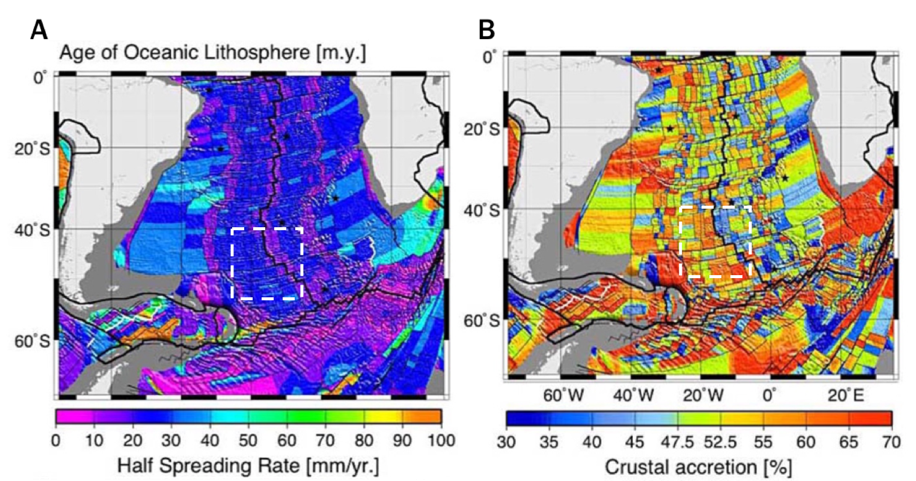
\includegraphics[width=0.9\linewidth]{./figs/hsr_muller.png}
	\caption{\textbf{A.} Seafloor half-spreading rates. \textbf{B.} Crustal accretion asymmetries in the South Atlantic, Scotia Sea, and northern Weddell Sea. Dashed boxes in A and B mark the region clearly showing asymmetric features. Modified from \citet{Muller2008}}
	\label{fig:hsr_muller}
\end{figure}

These previous studies have assumed the accretion of oceanic lithosphere at spreading centers to occur symmetrically and at a constant rate, but this assumption is not consistent with various observations \citep{Castelino2016, Flament2014, Martinez2006, Muller1998, Muller2008, Fedotova2017}. \citet{Castelino2016} explained anomalous bathymetry of the Mozambique basin and Riiser Larsen sea with the presence of thicker-than-usual oceanic crust older than 100 Ma. \citet{Flament2014} suggested that viscous lower mantle flow may represent topographic asymmetry of the South Atlantic. \citet{Martinez2006} identified non-corresponding trends in crustal thickness and spreading rate along the back-arc Eastern Lau Spreading Center. \citet{Muller2008} published global models for seafloor ages, spreading rates, and spreading asymmetry of ocean crust. If the two plates grew symmetrically at every divergent boundary, the spreading rates of the two plates would be the same and therefore relative proportions of crustal accretion on conjugate ridge flanks would be 50\% everywhere. However, their models clearly exhibit asymmetries in spreading rates and crustal accretion. For instance, in the South Atlantic region displayed on Figure \ref{fig:hsr_muller}, the different values of half-spreading rates and crustal accretion between left and right plates from spreading center are visible. The asymmetric plate growth is not specific to a particular region: It is a worldwide feature.
%
\begin{figure}[!htb]
	\centering
	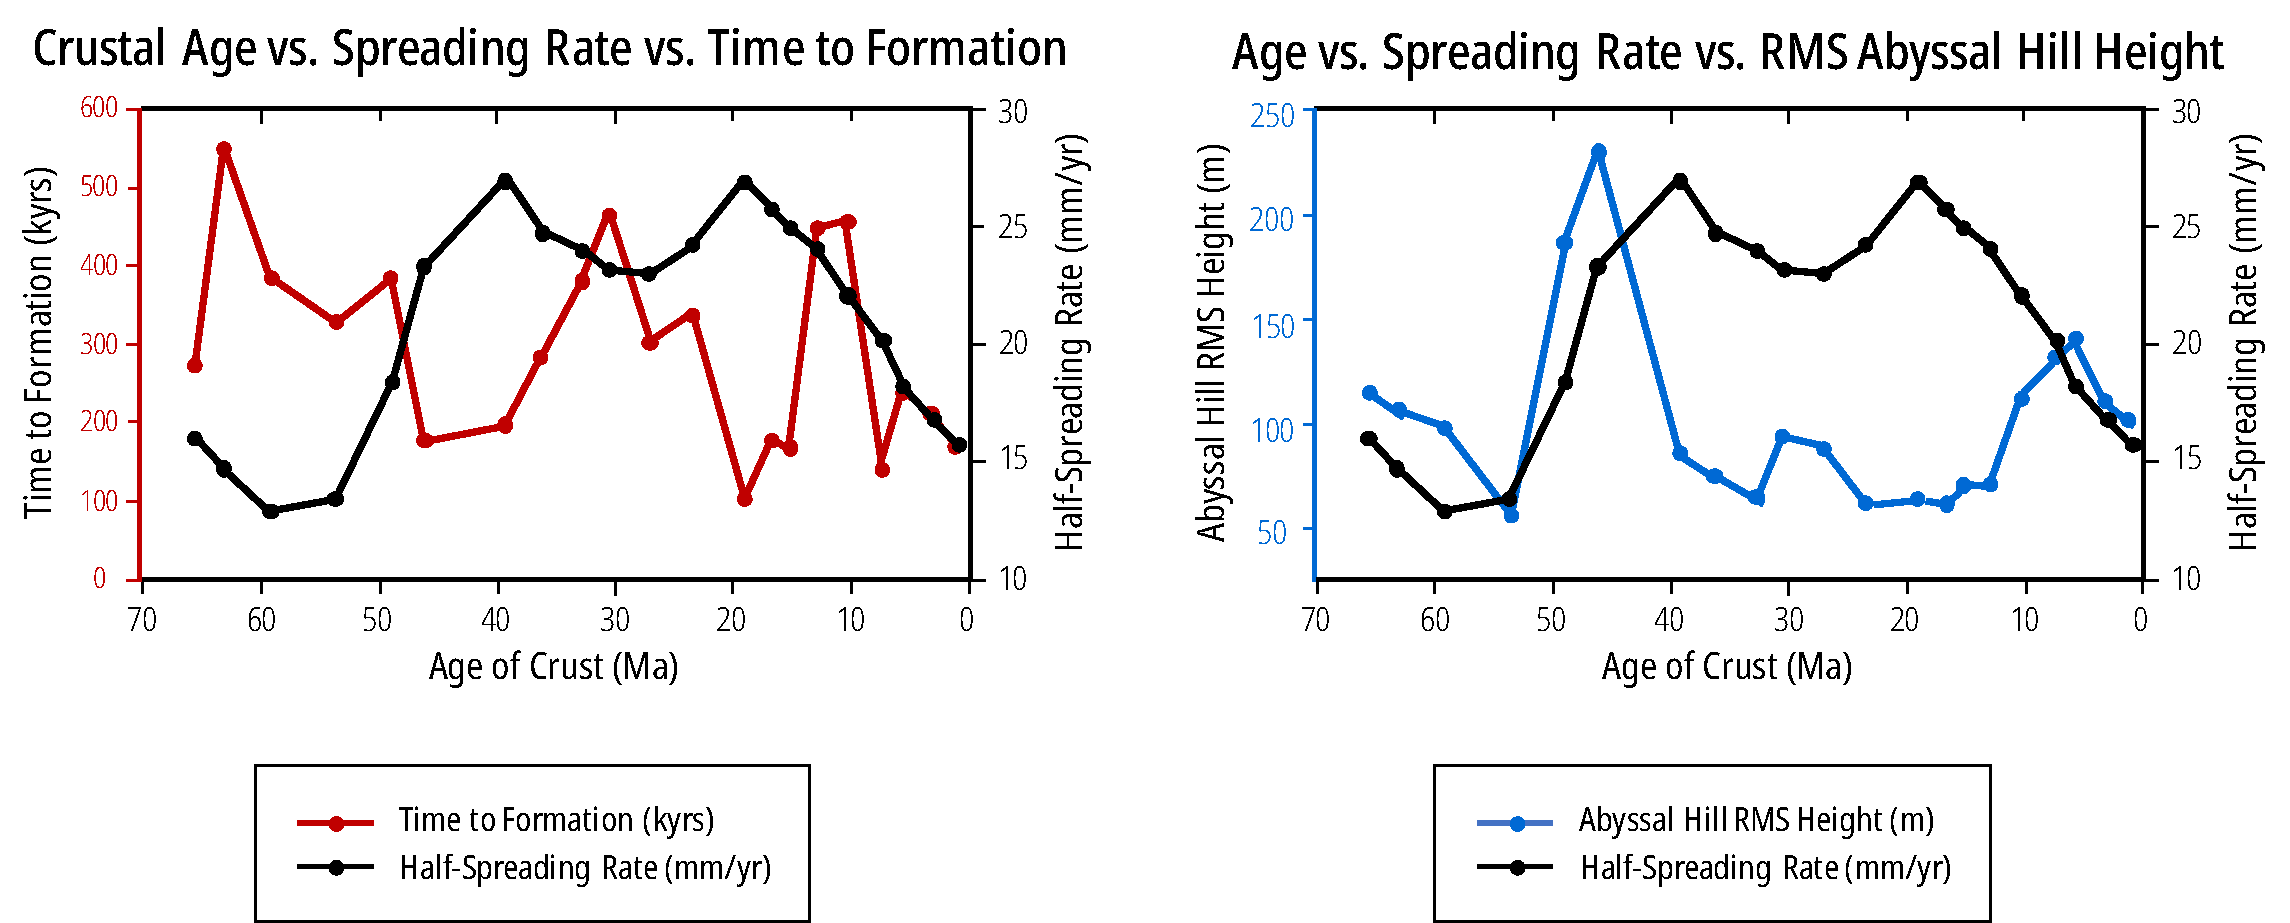
\includegraphics[width=0.99\linewidth]{./figs/hsrgraph1.pdf}
	\caption{Non-uniform half-spreading rate, abyssal height and time to form abyssal hill data from CREST expedition in mid-Atlantinc Ridge. Digitized from \citet{Fedotova2017}}
	\label{fig:hsr_fedotova}
\end{figure}

The rate of plate grow is not only asymmetric across divergent boundaries but variable in time as the data collected by the CREST (Crustal Reflectivity Experiment Southern Transect) expedition showed~\citep{Fedotova2017}. The collected data include half-spreading rates, times taken to form abyssal hills and abyssal hill heights. If plates grew at a constant rate, spreading rates and required times to form abyssal hills would be constant and byssal hill heights would be plotted as a sinusoidal curve with regular amplitude and frequency by assuming uniform plate spreading. However, the CREST data show significant variations in these observables over time (Figure \ref{fig:hsr_fedotova}). For instance, spreading rate varies by 15 mm/yr over the period of about 70 Myrs. Taken time to form abyssal hill varies by 450 Kyrs over the period of about 70 Myrs. These observations indicate non-uniform plate growing behavior on the seafloor.

Continental rifts, another type of divergent plate boundary, has recently been shown to form slowly during the incipient stage and accelerate later \citep{Brune2016}. Based on the kinematic modeling based on plate motion inversion data from the major passive margins of North Atlantic, North America – Greenland, Australia – Antarctica, and the South China sea, \citet{Brune2016} identified several rapid changes in absolute plate motion from the extension records in the major passive margins around the world, which have not been explained previously. They explained the multi-phase rifting as a result of the interaction between the rift-intrinsic strength and forces pulling the plates apart. At the initial stage of rifting, the lithosphere is still thick and strong and thus high strength lets rifting slow (Figure \ref{fig:brune}A). When the lithosphere gets significantly thinned and weakened, low strength enables fast rifting (Figure \ref{fig:brune}B).
%
\begin{figure}[!htb]
	\centering
	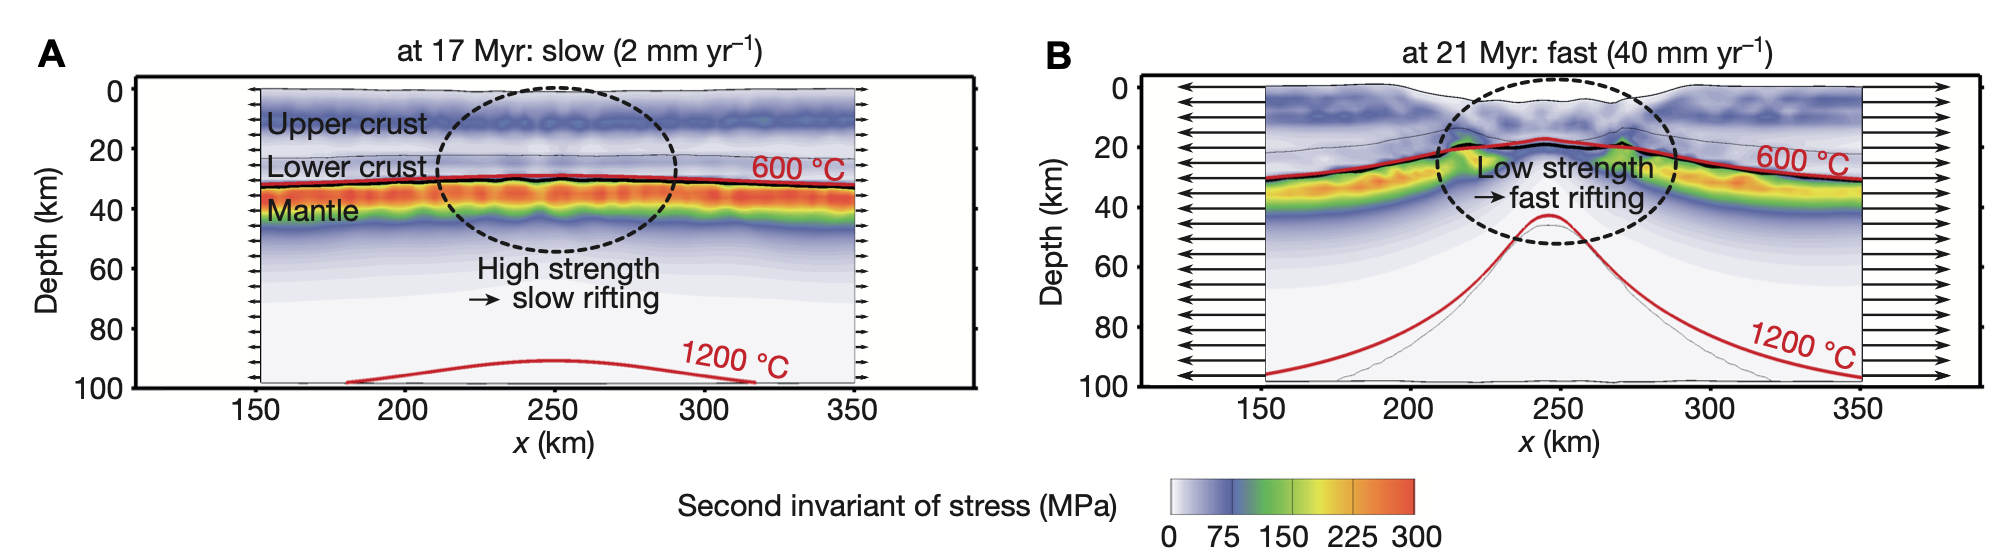
\includegraphics[width=0.99\linewidth]{./figs/brune.png}
	\caption{Strength evolution in numerical models for continental rifting with constant force boundary conditions. \textbf{A.} Distribution of the second invariant of stress at 17Myr when the lithosphere is still thick and strong and thus the extension rate is low, 2mm/yr. Arrows indicate extension velocity. \textbf{B.} After 21Myr when the lithosphere gets significantly thinned and weakened, letting the extension rate increase to 40 mm/yr. From \citet{Brune2016}}
	\label{fig:brune}
\end{figure}

Prompted by the non-uniform plate growth at mid-ocean ridges and potential interactions between the far-field forces and mid-ocean ridge processes, I investigate the mechanism of interactions between plate driving forces and internal forces at mid-ocean ridges, including diking and faulting using numerical models. Conventional kinematic boundary conditions are replaced with tractions in numerical models for mid-ocean ridges. I also include magmatic intrusion and faulting at a spreading center in models because magmatism and faulting play a vital role in determining characteristics of mid-ocean ridges. 

\chapter{Modeling Method}

Magmatism at the spreading center of mid-ocean ridges plays an essential role in determining faulting styles that in turn control the axial and seafloor morphology. At fast-spreading ridges, copious magma rises and forms axial high (Figure \ref{fig:ridgebathymetry}A). With abundant magma, diking can occur frequently accommodating a significant portion of plate separation. For this reason, faults forming near axial highs have only small (i.e., 100s m) offsets (Figure \ref{fig:ridgebathymetry}A). Density variations are significant across fast-spreading ridges since the axial lithosphere is very thin, hot, and underlain by partially molten crust. Axial highs might originate from fluid magma rising to the level of local isostatic equilibrium at the plate spreading axis and then subsiding as it cools down. In contrast, faults forming at slow-spreading centers show greater offset, and axial valleys form at the spreading center (Figure \ref{fig:ridgebathymetry}B). Less abundant magma compared to fast-spreading ridges means less frequent diking and tectonic stretching accommodates a significant portion of plate separation. Faults at slow-spreading ridges develop offset up to 1-2 km. Abyssal hills produced at slow-spreading ridges are composed of faults dipping towards the axis while about half of the faults near fast-spreading centers dip toward the axis and the other half dip away from ridge axis.

\begin{figure}[!htb]
	\centering
	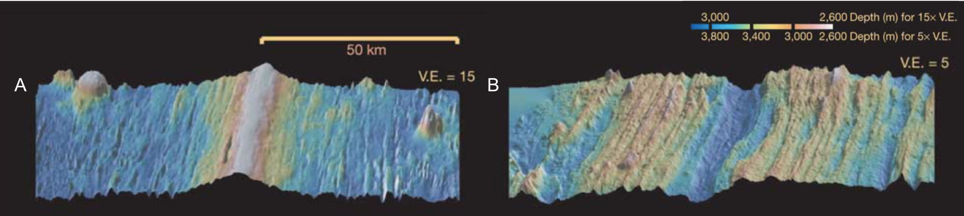
\includegraphics[width=0.99\linewidth]{./figs/bathy_buck.png}
	\caption{Shaded relief images of bathymetry at slow and fast ridges. \textbf{A.} The East Pacific Rise along 9$^\circ$37$'$N latitude \textbf{B.} The Southeast Indian Ridge along the 115$^\circ$E segment. Modified from \citet{Buck2005}.}
	\label{fig:ridgebathymetry}
\end{figure}

Assuming a constant magma injection rate at dike zone, \citet{Buck1998} simplified the complex diking process. They treated intrusion of a dike of low viscosity magma by specifying the stress on a vertical interface placed at the center of crust layer. Normal stress is set equal to the lithostatic pressure in crust layer and shear stress is set to zero on the interface.
This approach allowed the lateral position of a modeled dike to explain the contrasting faulting styles at slow- and fast-spreading ridges.

\begin{figure}[!htb]
    \centering
    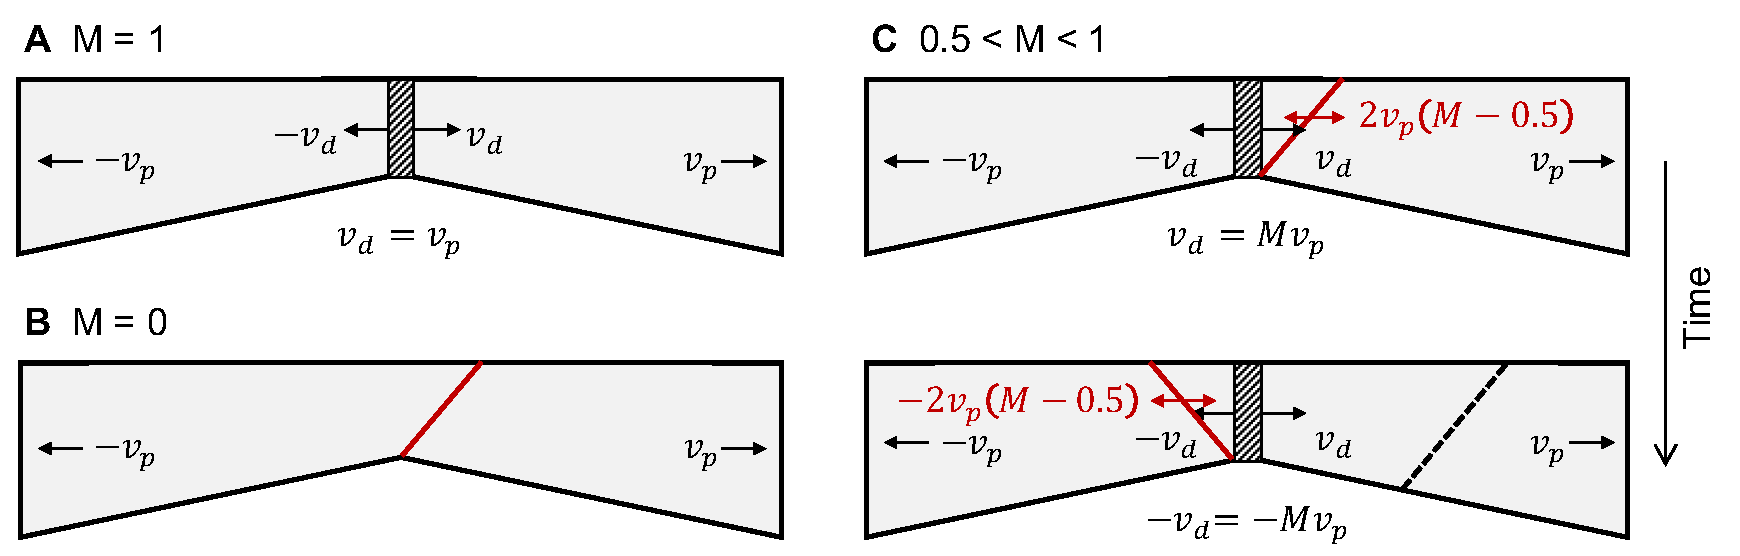
\includegraphics[width=0.99\linewidth]{./figs/mfactor.pdf}
    \caption{Cartoon showing how M factor determine plate separation mechanism. \textbf{A.} M = 0, all extension is taken up by fault. No diking occurs. \textbf{B.} M = 1, dike accommodates all extensions. Dike opening rate and plate separation rate are same. \textbf{C.} 0.5 $<$ M $<$ 1, more than half of plate separation is accommodated by dike and hence faults migrate off axis. It shows how the hanging-wall block of a fault may migrate during ridge stretching.}
    \label{fig:mcartoon}
\end{figure}

\citet{Buck2005} introduced the ratio of dike opening rate to total plate spreading rate as a parameter for numerical mid-ocean ridge models. This ratio is denoted as M and when given as a parameter for a model, it determines the rate of diking-accommodated plate separation as M times total spreading rate. When M = 0, dikes account for none of the plate spreading (Figure \ref{fig:mcartoon}A); and dikes accommodate all the plate separations when M = 1 (Figure \ref{fig:mcartoon}B). M less than one corresponds to the case where magma supply is insufficient for filling the entire opening created by plate separation and tectonic stretching of the lithosphere should occurs. For M = 1, axial lithospheric separation is all taken up by dike widening and no faults or axial valleys develop.  For 0.5 $<$ M $<$ 1, faults develop and slip at a horizontal rate of 2$v_p$ (M $-$ 0.5) (Figure \ref{fig:mcartoon}C). Since the opening by diking is faster than the rate that the fault offset increases, the fault itself is pushed off axis with time. When pushed far away from the axis, the fault locks because the lithosphere around the fault becomes thicker and stronger. As a result, a new fault forms at the spreading center, continuing to accommodate a part of plate separation. For M = 0, dikes account for none of the plate spreading. Results for stretching-dominated ridge models are illustrated in Figure \ref{fig:mfactor}A and B. In the case of M = $\sim$1, the model produces a symmetric pattern of small-offset faults, producing a bathymetric profile similar to that of the Southeast Indian Ridge (Figure \ref{fig:mfactor}A). For M = 0.5, the model generates two large offset faults on one side, and a series of small faults on the other side. Lithospheric stretching creates conjugate normal faults at the spreading center initially. Only one branch survives on one side of the ridge, eventually evolving into a detachment fault, while short-lived new faults semi-regularly form on the opposite side. The resultant bathymetric profile resembles that of the slow-spreading Mid-Atlantic Ridge (Figure \ref{fig:mfactor}B).
%
\begin{figure}[!htb]
	\centering
	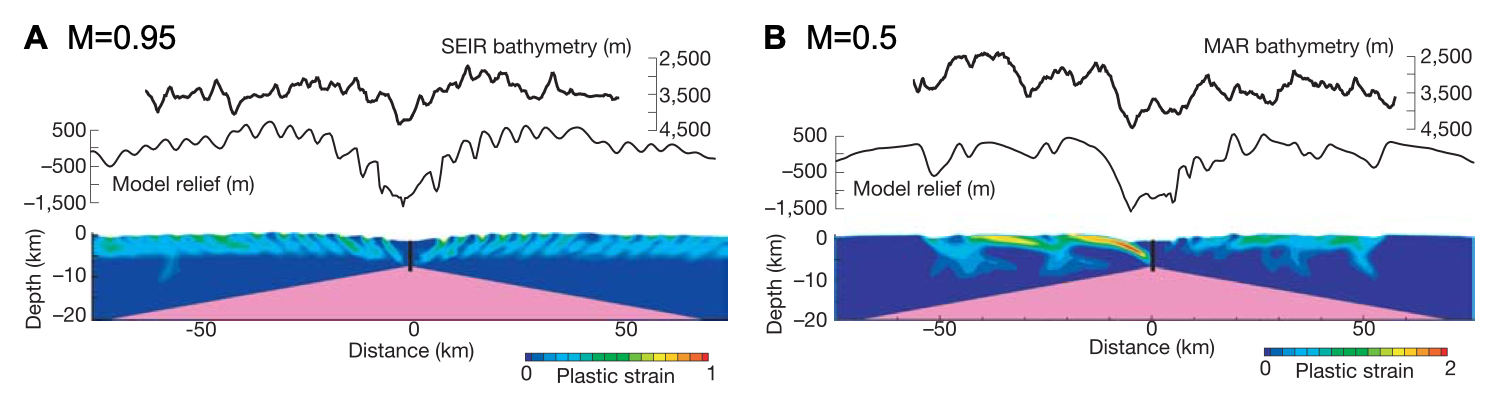
\includegraphics[width=0.99\linewidth]{./figs/fig1.png}
	\caption{\textbf{A.} Plastic strain distribution and surface relief from the numerical model with M = 0.95. High plastic strain represents shearing on faults and the bathymetric profile across the Southeast Indian Ridge (SEIR) is shown for comparison. \textbf{B.} Same as \textbf{A} but for M = 0.5. A bathymetric profile from the Mid-Atlantic Ridge (MAR) is shown for comparison. From \citet{Buck2005}}
	\label{fig:mfactor}
\end{figure}

%\section{Numerical approach}
%\note[EC]{Let's reorganize ``Numerical approach'' as follows: Governing equations, Numerical methods for approximate solution. Then, ``Model Setup'' becomes a new (sub-)section.}

%\section{Governing equation}
%mass balance equation
%\begin{align}
% \frac{\partial \rho}{\partial t} + \nabla \cdot (\rho \mathbf{v}) = 0
%\end{align}
%
%linear momentum balance equation
%\begin{align}
%\nabla \cdot \boldsymbol{\sigma} + \rho \mathbf{b} = \rho \frac{D \mathbf{v}}{Dt}
%\end{align}
%
%energy balance equation
%\begin{align}
%\rho C_{p} \frac{\partial T}{\partial t} = k \nabla^2 T
%\end{align}
%
%and constitutive equation for a non-Newtonian fluid

\section{Observed bathymetry and faulting modes \note[EC]{Does this topic deserve a separate section? Also, relate these back to the M factor models.}}
Oceanic core complexes(OCCs) have been recognized along slow- and ultraslow- spreading ridges \citep{Tucholke1998}, and are characterized by dome-shaped bathymetric highs interpreted as portions of the lower crust and/or upper mantle exposed by detachment faulting \citep{Tucholke1994}. OCCs form at or near the axis, beneath long-lived ($\sim$1-2 Myr) normal faults which are commonly observed on mid-ocean ridges. Figure \ref{fig:occ} shows an observed detachment fault in multibeam bathymetry data. Detachment locates at near 37 km distance with $\sim$3000 m offset.
%
\begin{figure}[!htb]
	\centering
	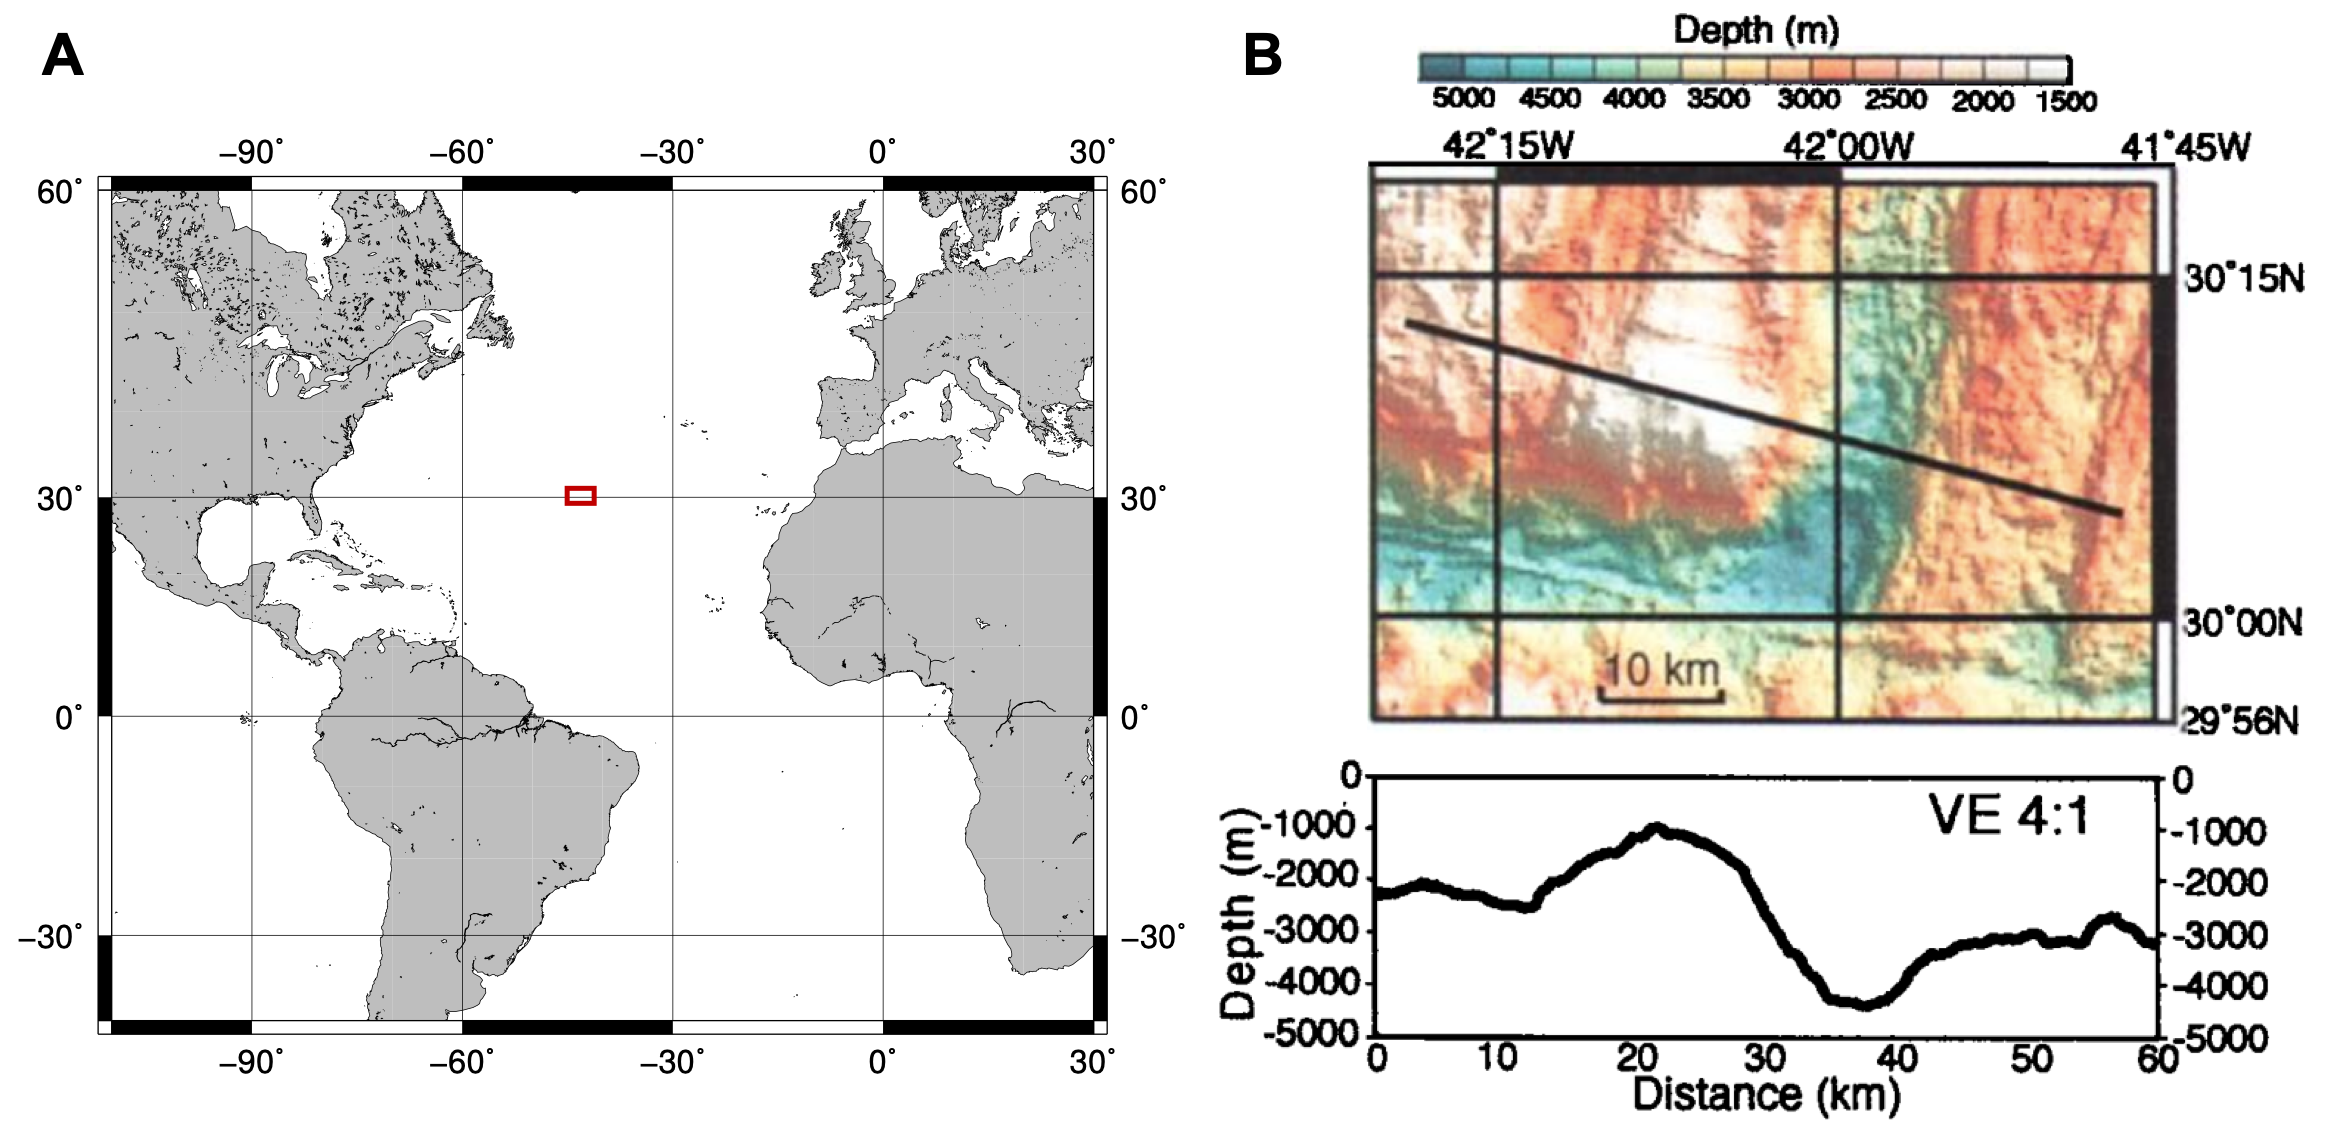
\includegraphics[width=0.6\linewidth]{./figs/occ.png}
	\caption{Multibeam bathymetry data of Mid-Atlantic Ridge (MAR) gridded at 200m spacing (RIDGE Multibeam Synthesis). Topographic profile along estimated direction of spreading shows detachment fault. From \citet{Lavier2000}}
	\label{fig:occ}
\end{figure}
%

Abyssal hills form at mid-ocean ridge spreading centers by magmatism and normal faulting that occurs alternatingly on both sides of the ridge axis. Figure \ref{fig:abyssalhill}A shows multibeam bathymetry data \add[EC]{for XXX ridge, where abyssal hills are observed and explained as a product of alternating small-offset normal faults}. Figure \ref{fig:abyssalhill}\annote[EC]{C and D}{What about B? You should show more care with explaining figures. I\rq{}ve said this many times but you shouldn\rq{}t just throw a figure at readers: You have to engage in explaining what is being shown and why you are showing it}. point out the feature of abyssal hills, the offsets of the faults are much smaller than that of detachment fault.
%
\begin{figure}[!htb]
	\centering
	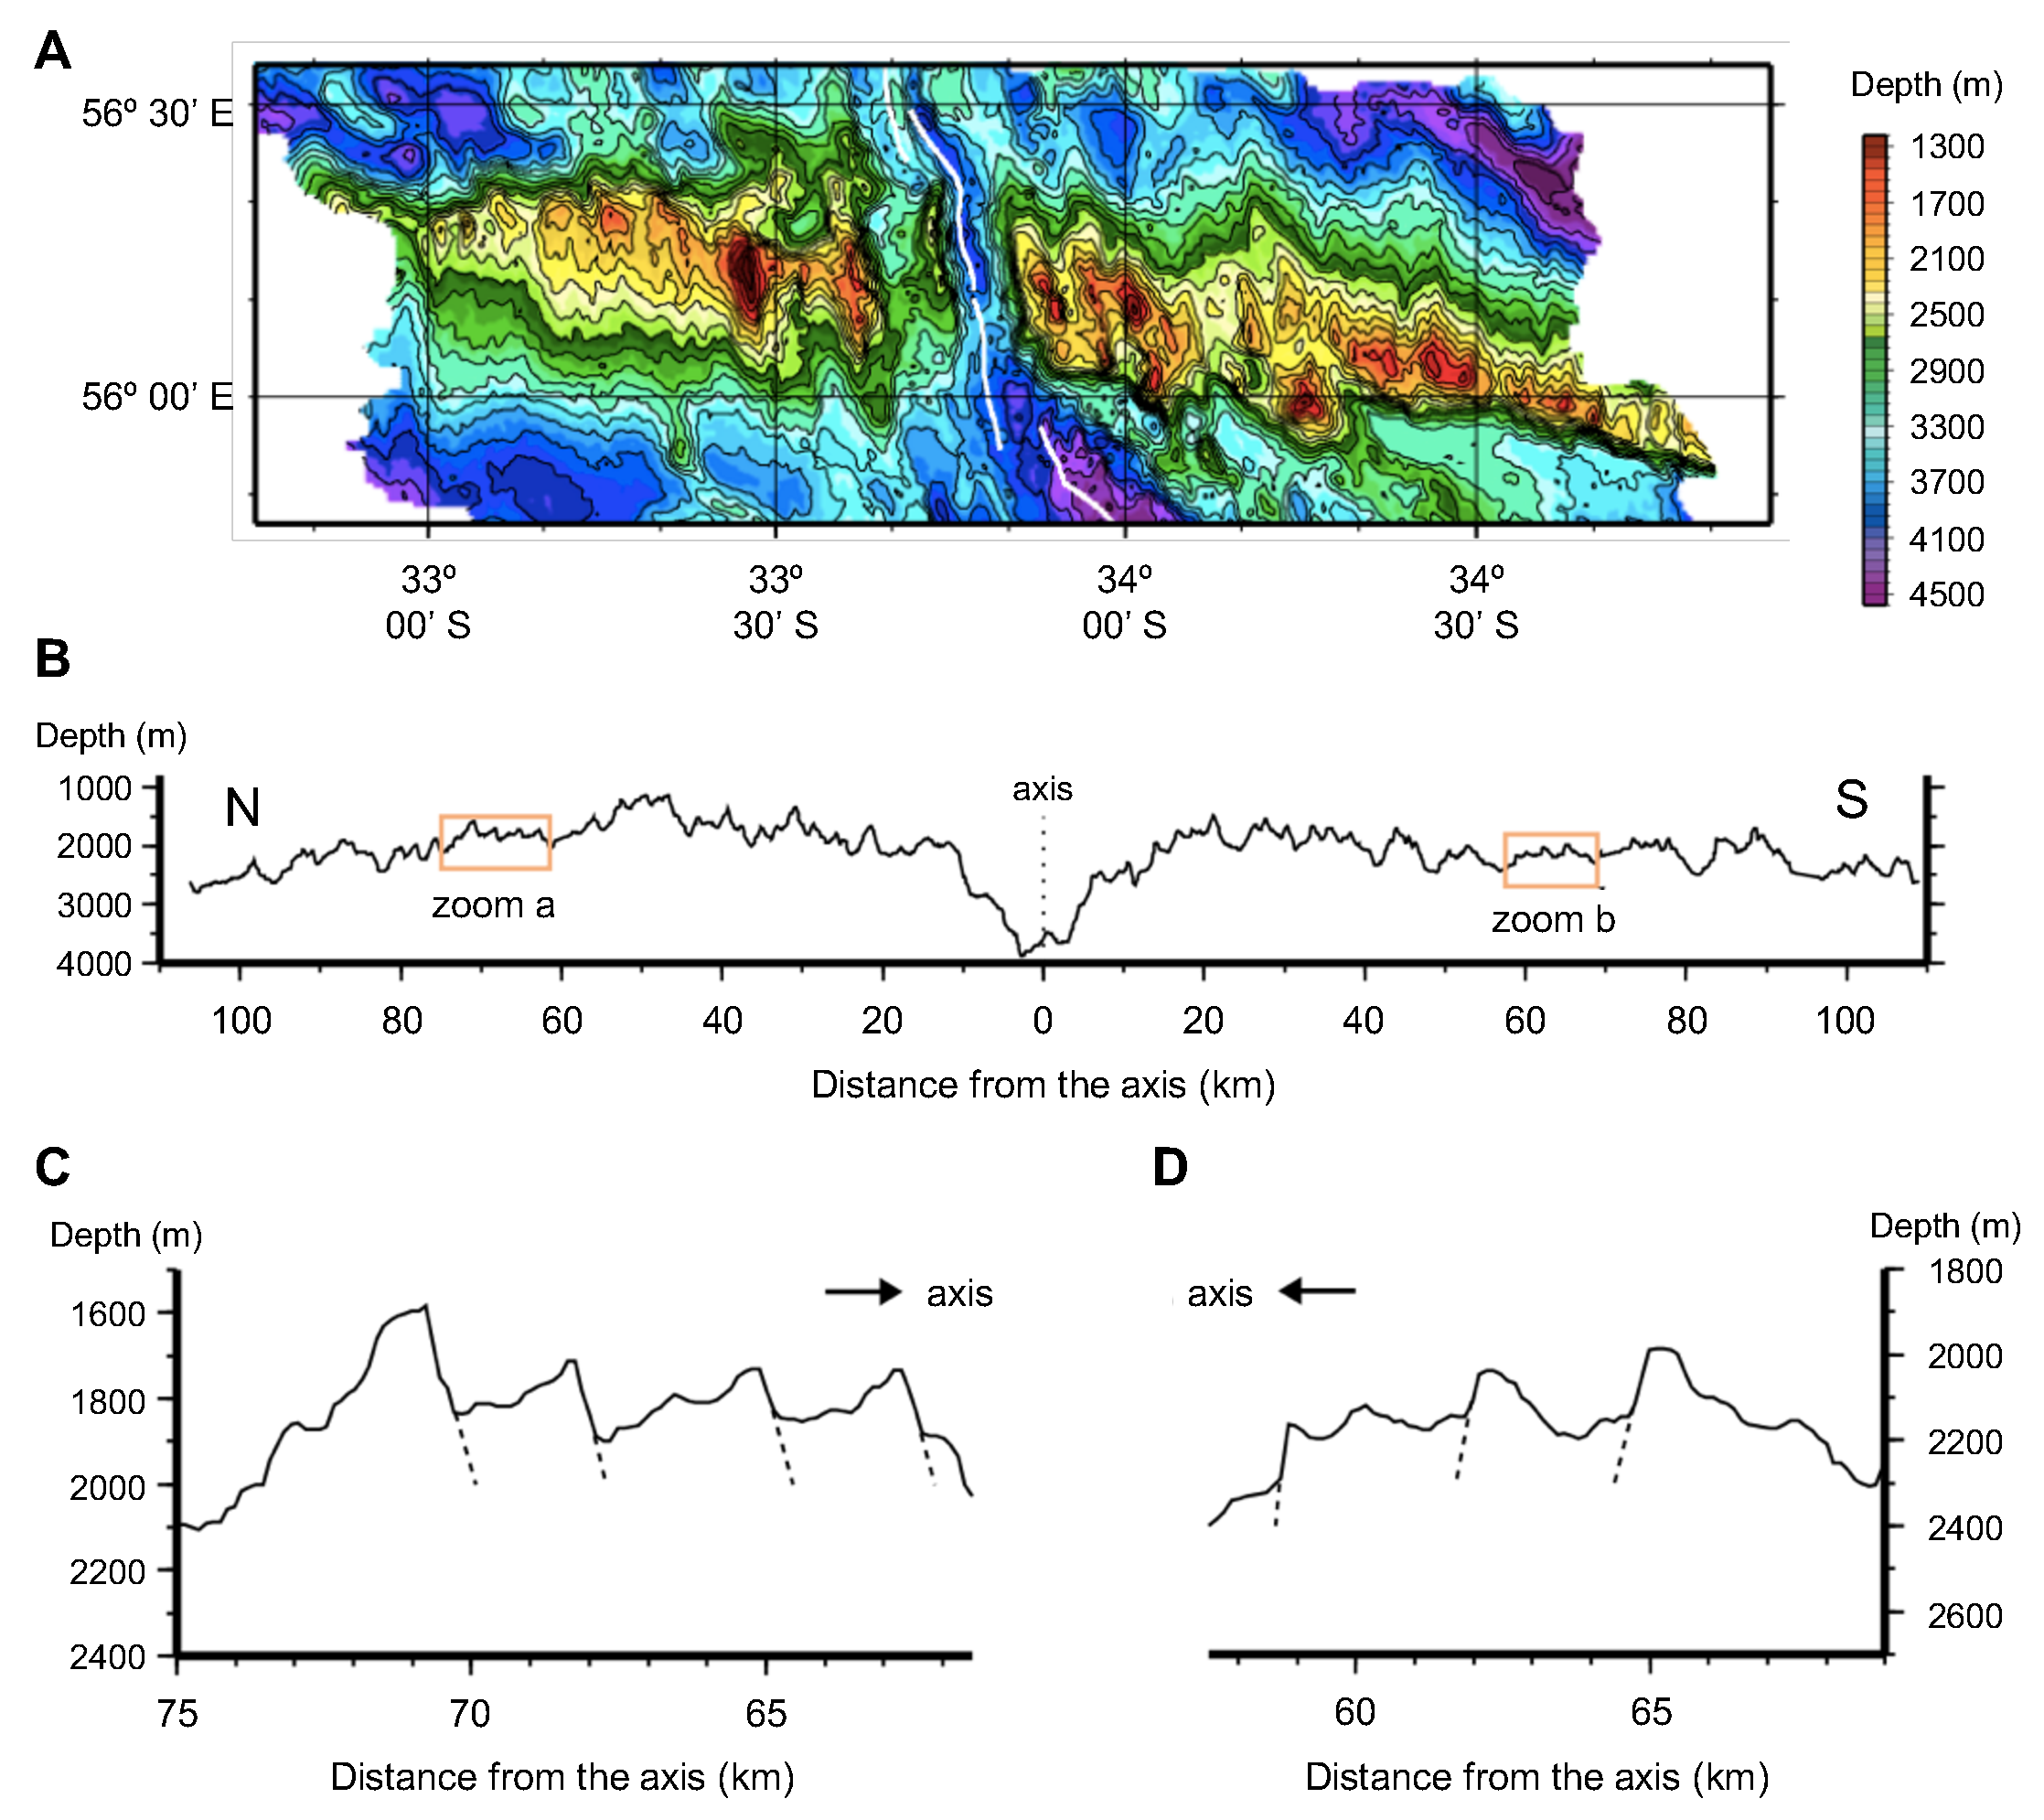
\includegraphics[width=0.98\linewidth]{./figs/abyssalhill.pdf}
	\caption{\textbf{A.} Multibeam bathymetric data of the Southwest Indian Ridge (SWIR). White line is the ridge axis. \textbf{B.} Bathymetric cross sections along the spreading direction of abyssal hills of \textbf{A}. \textbf{C.} Enlargement on 'zoom a'. Dashed line is fault surface. \textbf{D.} Same with \textbf{C}, but on 'zoom b'. Modified from \citet{Mendel2003}}
	\label{fig:abyssalhill}
\end{figure}
%

\section{Numerical methods for approximate solution}
FLAC (Fast Lagrangian Analysis of Continua) method \citep{Cundall1982, Poliakov1993} solves the equations describing conservation of momentum and energy for a visco-elastic-plastic continuum in 2-D Cartesian geometry \citep{Lavier2002}. By solving the conservation of momentum, the accelerations are integrated in time to give updated velocities, strains and strain rates. In addition, using the constitutive laws the strains and strain rates are used to calculate new elastic and viscous stresses. These stresses are used to determine the accelerations for the next step of calculation. The FLAC code that I used for this study is available at \url{https://github.com/heec12/non-uniform_plate_growth}. Also, the input parameter files necessary for reproducing the results presented here are available.

\section{Model Setup}
Materials in my mid-ocean ridge models are assumed to be elasto-visco-plastic. In this rheology, the brittle behavior is modeled by strain-weaking elasto-plasticity and the ductile behavior is modeled by Maxwell visco-elasticity. \note[EC]{If the Maxwell viscoelastic unit diagram is so important as for you to show it here, add a proper caption and spend more efforts to described it. Otherwise, don\rq{}t show the figure.}
%
\begin{figure}[!htb]
	\centering
	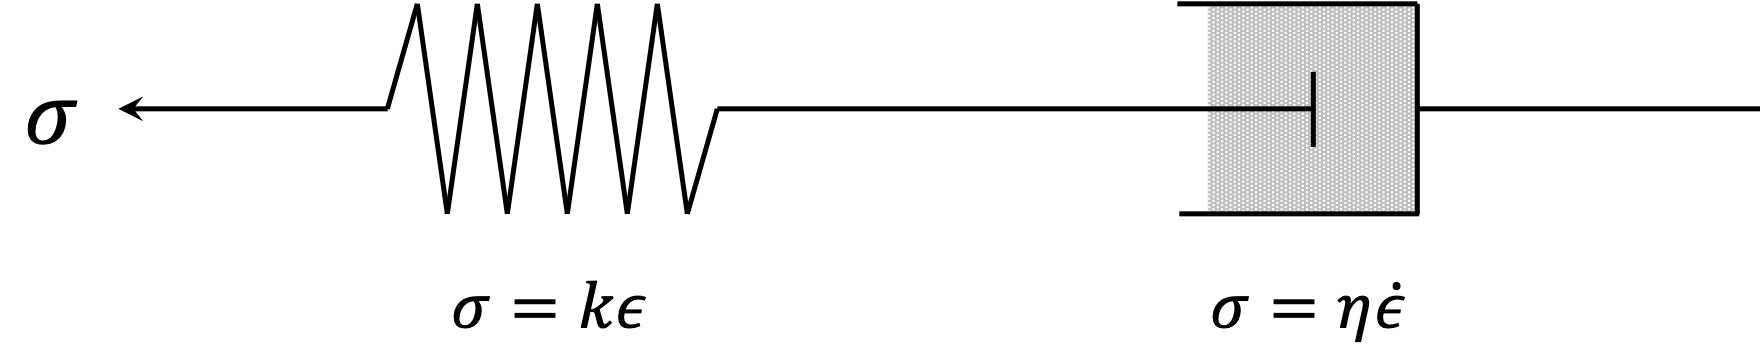
\includegraphics[width=0.6\linewidth]{./figs/maxwell.png}
%	\caption{}
	\label{fig:maxwell}
\end{figure}
%
For visco-elastic deformation, the linear Maxwell viscoelastic model is adopted, in which strain rates are assumed to be the sum of elastic and viscous strain rates \note[EC]{Why the subscript `s\rq{} and `d\rq{}? Also, make sure to explain all the symbols introduced as you did for the equation for the yield stress. The same goes with the viscosity formula.}.
\begin{align} \label{srate}
  \dot{\epsilon} &=  \dot{\epsilon_s} +  \dot{\epsilon_d} \\
                        &= \frac{ \dot{\sigma}}{k} + \frac{\sigma}{\eta}
\end{align}
Viscosity is determined by the dry diabase power law rheology~\citep{Kirby1987, Chen1990}.
\begin{align} \label{Visc}
 \eta = \frac{1}{4} \bigg( \frac{4}{3A} \bigg)^{1/n} \dot{\epsilon}^{(1/n)-1} \exp\bigg(\frac{Q}{nRT}\bigg)
\end{align}

Plastic yielding is controlled by the strain-weakening Mohr-coulomb plasticity model. In this model, the yield stress is determined as
\begin{align}
 \tau = \mu \sigma_n + C,
\end{align}
where $\tau$ and $\sigma_{n}$ are shear and normal stress, $\mu$ is friction coefficient and $C$ is cohesion.
%
Strain weaekning is realized by decreasing cohesion with the total accumulated plastic strain while friction coefficient is assumed to be constant~\citep{Poliakov1998}. In this study, cohesion decreases linearly from its initial value 44 MPa to the minimum value of 4 MPa.
%
\begin{table}[h!]
	\centering
	\caption{Summary of model parameters}
	\label{tab:modelparams}
	\begin{tabular}{cccc}
		\toprule
		Variable & Description & Value & Units\\
		\midrule
          	$\lambda$ & Density & 3300 & $kg/m^3$\\
	        n & From Eq \ref{Visc} & 4.7 & \\
	        A & From Eq \ref{Visc} & 190 & \\
	        E & Activation energy & 4.85e+5 & $kJ/mol$ \\
	        $\lambda$ & 1st Lam\'e parameter & 12 & GPa\\
	        $\mu$ & \annote[EC]{Shear modulus}{But the symbol is also used for friction coefficient. Straighten this out.} & 12 & GPa\\
	        $C_{max}$ & Maximum cohesion & 44 & MPa\\
	        $C_{min}$ & Minimum cohesion & 4 & MPa\\
		\bottomrule
	\end{tabular}
\end{table}
%
\begin{figure}[!htb]
	\centering
	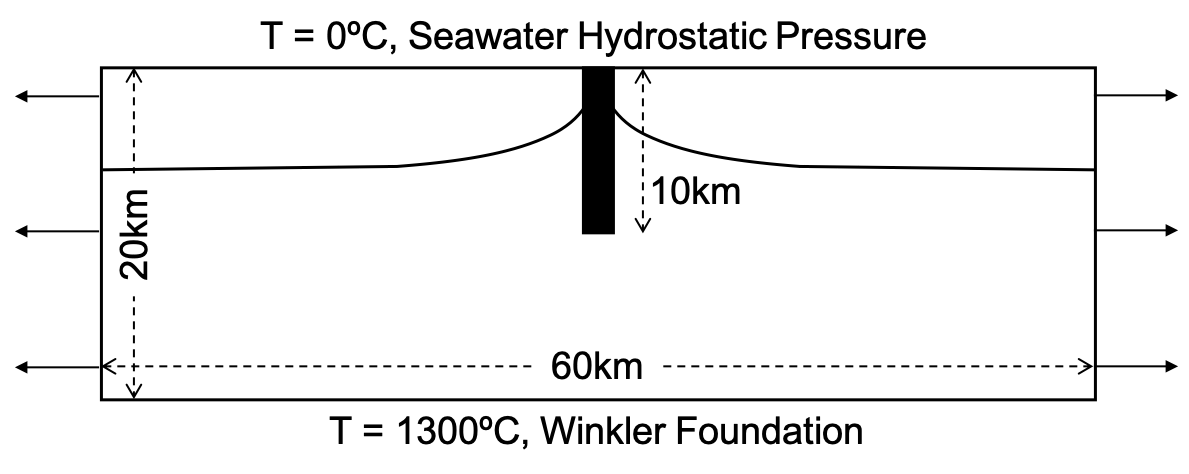
\includegraphics[width=0.8\linewidth]{./figs/modelsetup.png}
	\caption{Model setup used for numerical simulations of mid-ocean ridge system. For both velocity- and force-driven model, same initial and thermal boundary conditions are applied.}
	\label{fig:modelsetup}
\end{figure}
%

The model domain is rectangular with a ridge axis at the center. All the models have 60 km wide and 20 km deep of domain sizes with the grid of 0.5 $\times$ 0.5 km. At the top boundary, I apply seawater hydrostatic pressure while Winkler foundation is assumed for the bottom side (Figure \ref{fig:modelsetup}).

Building on this common basis, I explore how oceanic plates grow when plate motions are driven by forces applied on the boundary rather than by prescribed kinematics. Three cases with an increasing order of complexity are considered.

\subsection{Case I: Kinematic models}

Plate motions are driven by prescribed velocities on the left and right boundaries at a rate of 2.5cm/yr. The purpose of this traditional approach is to verify that the faulting modes are reproduced as in the previous studies \citep{Buck2005,Tucholke2008}.

\subsection{Case II: $(\boldsymbol{F_{res}})_x \mathbf{=0}$ models}

Plate motions are assumed to occur as a result of the balance between three forces acting on plates (Figure \ref{fig:forcescheme}): (1) Boundary force ($\mathbf{F}_{bdy}$) applied at the two side boundaries of lithosphere; (2) brittle force ($\boldsymbol{F}_{brt}$) arising as lithophere is elastically stretched, creates faults and keeps them active; %or forms faults a counter force to $F_{bdy}$ in the opposite direction; 
and (3) viscous force ($\boldsymbol{F}_{vis}$) required for lithosphere to drag asthenosphere along. 
%Additionally, the force from faulting and its evolution is called fault force ($\boldsymbol{F_{fault}}$). 
For later purposes, the sum of the latter two is termed as an internal force ($\boldsymbol{F}_{int}$). Then, residual force ($\boldsymbol{F}_{res}$) can be defined as the sum of $\boldsymbol{F}_{bdy}$ and $\boldsymbol{F}_{int}$:
%
\begin{align} \label{Fres}
\mathbf{F}_{res} & = (\mathbf{F}_{brt} + \mathbf{F}_{vis}) + \mathbf{F}_{bdy} \\
 & = \mathbf{F}_{int} + \mathbf{F}_{bdy}.
\end{align}
%
\begin{figure}[!htb]
	\centering
	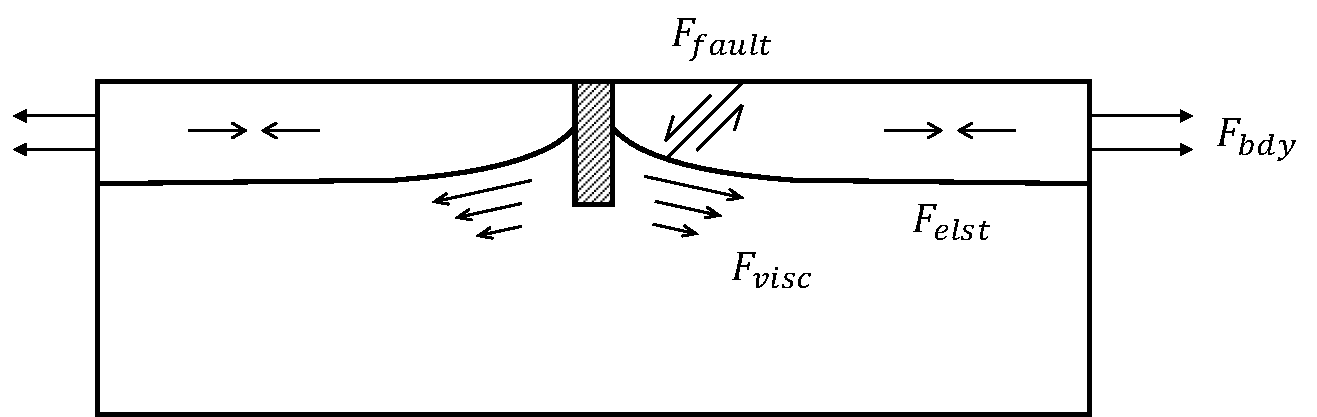
\includegraphics[width=0.9\linewidth]{./figs/force.pdf}
	\caption{Schematic illustration of the internal forces and boundary forces applying to the model.}
	\label{fig:forcescheme}
\end{figure}

Since $F_{int}$ is only a response to the boundary force and it is $F_{res}$ that determines how lithosphere accelerates, I control the magnitude of $F_{res}$ to initiate the motion of plates, which are at rest in the beginning, and maintain their speeds at a target value. Since $F_{int}$ would vary in time as faults grow or other changes occur in lithosphere and asthenosphere, controlling $F_{res}$, the sum of $F_{bdy}$ and $F_{int}$, implies that $F_{bdy}$ is automatically adjusted such that the sum with $F_{int}$ becomes the prescribed value. The boundary forces are in practice applied as traction (i.e., surface force per area) in my 2D models with the third dimension assumed to have the unit length. The code internally performs the surface integral of tractions to compute boundary forces.

The magnitude of the horizontal component of the residual force, $(\boldsymbol{F}_{res})_{x}$ is initially zero but linearly increases with time. Abrupt application of the residual force often causes the faults to form near the side walls rather than at the spreading center.
% the mean plate speed quadratically
To avoid undesirable boundary failure, I search for an appropriate rate of increasing $(\boldsymbol{F}_{res})_{x}$ with time by observing faulting behaviors for the values from 1 to 1000 Pa/yr (Table \ref{tab:slope}). When the plate speed reaches 2.5 cm/yr, I set the magnitude of $(\boldsymbol{F}_{res})_{x}$ to be zero in order to maintatin the velocity of the plate.
%
\begin{table}[h!]
	\centering
	\caption{Model results of 1Myr of spreading for $(\boldsymbol{F_{res}})_x$ incresing slope ranging from 1 to 1000 Pa/yr with two different M value. Expected model behavior for M=0.5 is a master detachment fault and alternating faulting for M=0.8}
	\label{tab:slope}
	\begin{tabular}{ccc}
		\toprule
		Slope, Pa/yr & M = 0.5 & M = 0.8\\
		\midrule
          	1 & Detachment fault forms 120 Kyrs later & Alternating faulting is visible\\
		10 & Detachment fault forms 100 Kyrs later & Faulting repeats only on right side\\
		100 & Detachment fault forms 81 Kyrs later & Alternating faulting mode, \\
		&&but faulting is dominanted on right side\\
		1000 & Boundary failure occurs & Boundary failure occurs\\
		\bottomrule
	\end{tabular}
\end{table}
%
%Setting $(\boldsymbol{F_{res}})_x$ as a zero after initial phase allow me to examine the expected physical behavior in force boundary applied model. 

\subsection{Case III: Constant ($\boldsymbol{F}_{bdy}$)$_x$ models}

Unlike Case II, this group of models have prescribed $x$ component boundary force, ($\boldsymbol{F}_{bdy}$)$_x$ on the boundareis of lithosphere. The net force resulting at the boundary nodes, $(\boldsymbol{F}_{res})$, is determined as the sum of $\boldsymbol{F}_{bdy}$ and time-evolving $\boldsymbol{F}_{int}$.

When M=0.8, \annote[EC]{the alternating faulting}{Did you explain this term earlier? If not, you will have to introduce this and the detachment faulting beforehand. You can refer to one of the earlier figures for the alternating faulting but none seems to show the detachment fautling. This explanation deserves a separate paragraph or a section because you can also clarify that faulting modes are the only characteristic you care about in this study. For instance, you are not going to compare the surface topography from a model with actualy bathymetry, right?} \add[HC]{See 'Observed bathymetry and faulting modes' section?} is expected~\citep{Tucholke2008}. The evolution of alternating faulting can be divided as three stages: incipient, mature and terminal stages. At the incipent stage (Figure \ref{fig:faultstage}A), new fault occurs on one side of the ridge axis. The fault heave increases and fault dip decreases as fault grows during the mature stage (Figure \ref{fig:faultstage}B). The terminal stage is characterized by the replacement of the locked fault by a new near-axis fault on the opposite side of ridge axis. 
%
\begin{figure}[!htb]
	\centering
	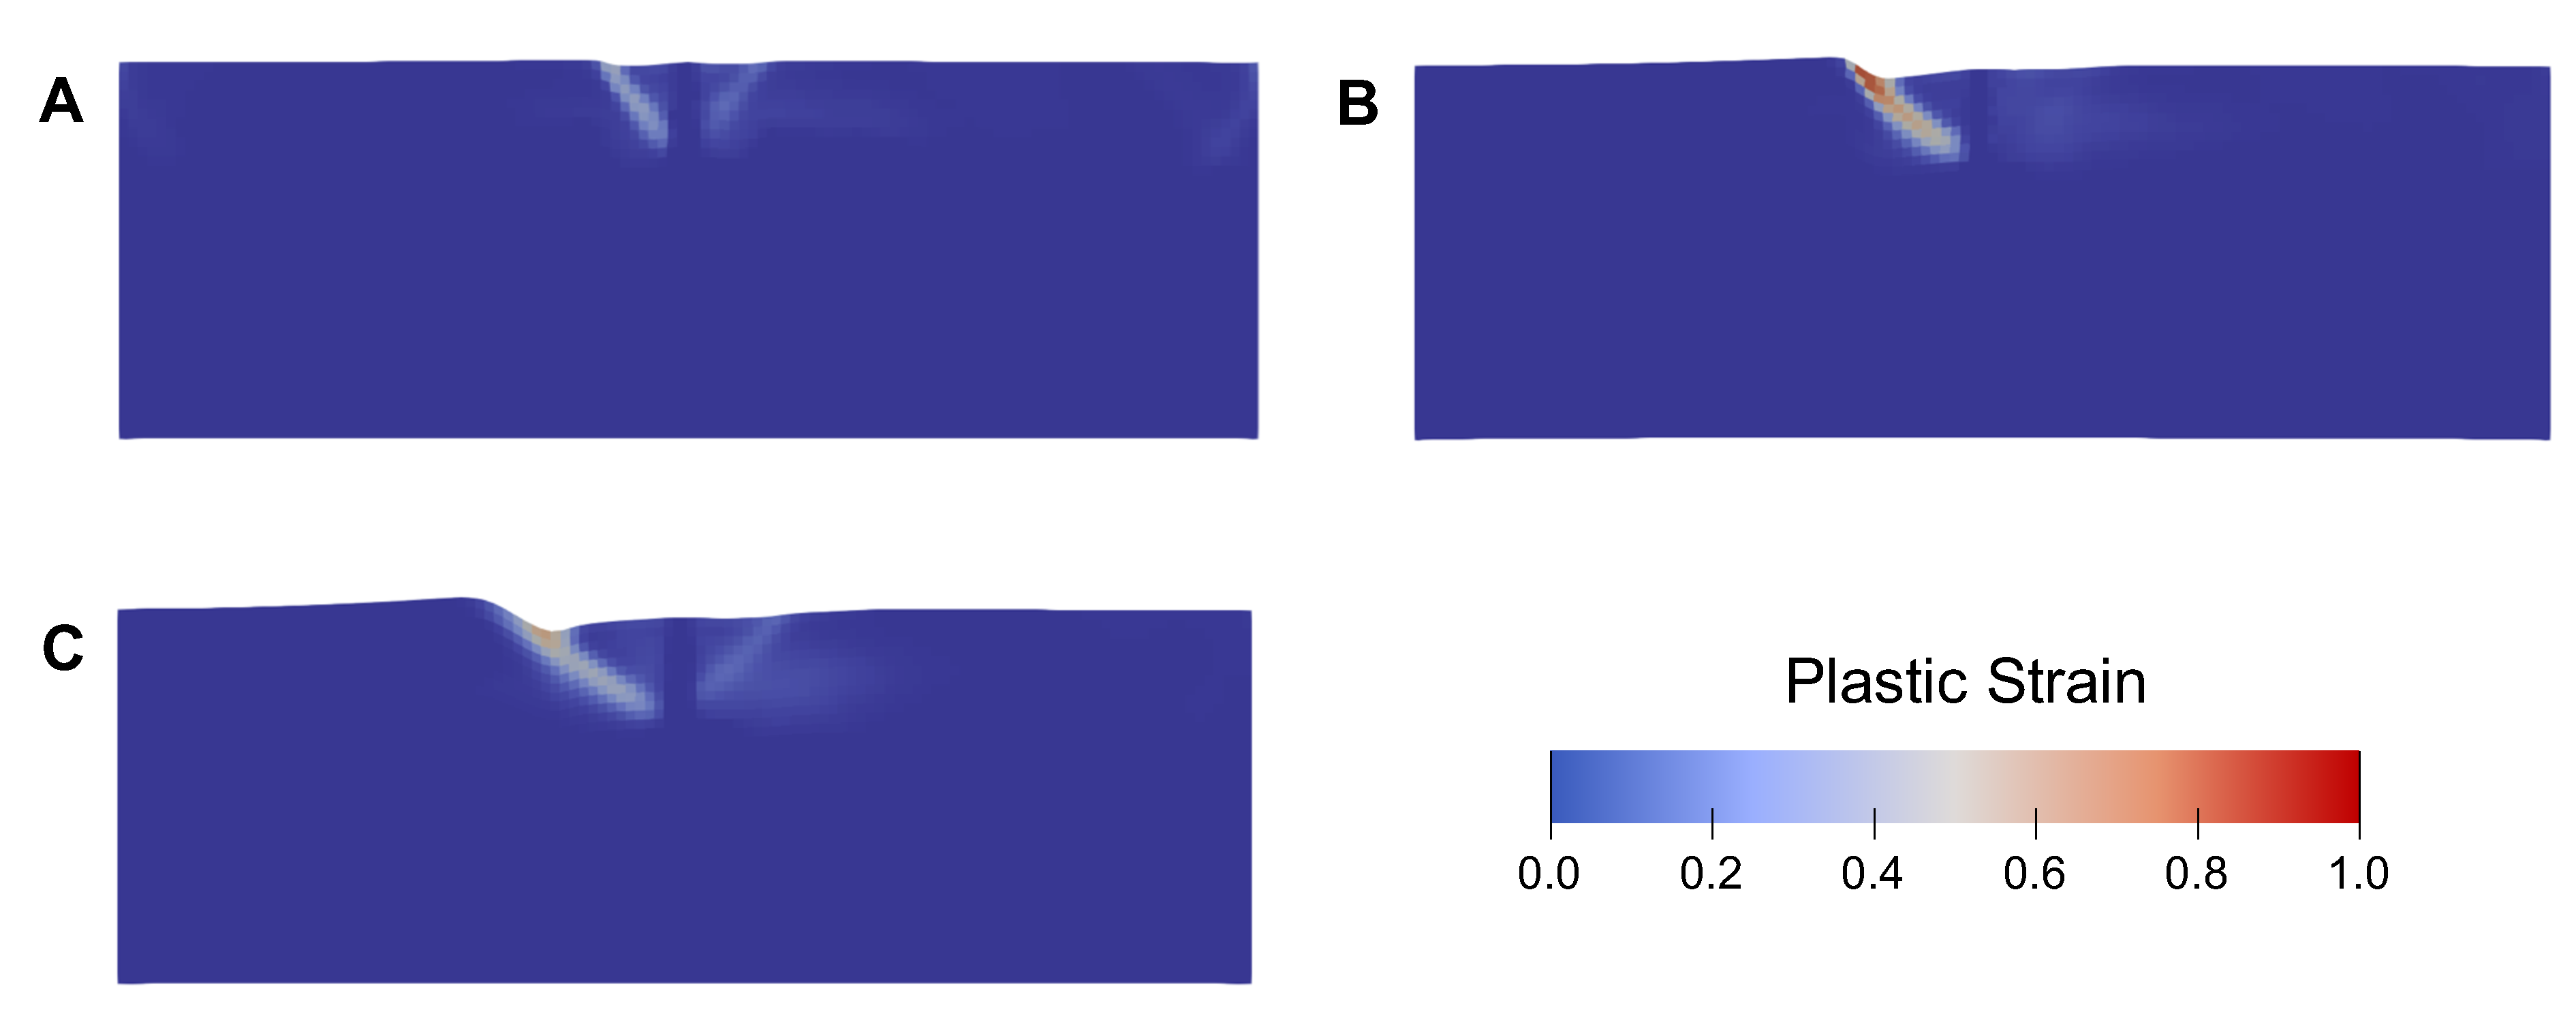
\includegraphics[width=0.9\linewidth]{./figs/fault_stage.pdf}
	\caption{Snapshots of the kinematic model (M = 0.8) representing stages of the fault evolution. The fault evolution can be divided as three stages. \textbf{A.} Incipient stage: new fault occurs on left side of the ridge axis. \textbf{B.} Mature stage: fault heave increases and fault dip decreases as fault grows. \textbf{C.} Terminal stage: fault becomes inactive and is replaced by a new-near axis fault on the other side of ridge axis.}
	\label{fig:faultstage}
\end{figure}

I assign to $(\boldsymbol{F}_{bdy})_x$ the value of time-averaged $(\boldsymbol{F}_{int})_x$ ($\overline{(\boldsymbol{F}_{res})_x}$) from \annote[EC]{a kinematic model}{Correct this.} with the same value of M. While a kinematic model with a desired value of M is run, $(\boldsymbol{F}_{int})_x$ values on all the nodes on the side boundaries are recorded. Those values of $(\boldsymbol{F}_{int})_{x}$ are then averaged over the period from the mature stage of the first fault to the incipient stage of the new fault on the opposite side.

I let $(\boldsymbol{F_{res}})_x$ be computed only on the nodes in the brittle state, in which I assume temperature is lower than 600 $^\circ$C \citep[e.g.,][]{Violay2012}. Assuming that the ductile mantle is only passively pulled up beneath the spreading center and dragged along by the brittle lithosphere, I set ($\boldsymbol{F}_{res}$)$_x$ of the ductile parts of the side boundaries to be zero. This treatment is equivalent to assumging that the boundary force is perfectly balanced with the viscous resistance on the ductile portions of the boundaries. %Most of tectonic activities have been shown to be a consequences of plate motions. Therefore, I apply the force only acting on brittle plates and let $(\boldsymbol{F_{bdy}})_x$ as a zero.

\chapter{Results}

\section{Kinematic models}

The kinematic models reproduce the faulting modes for each M value reported in the previous studies. In the M = 0.5 model, a normal fault forms by 0.1 My and remains active over the entire duration of the model, 1 My, producing an oceanic core complex (Figure \ref{fig:kfault_m05}). When M is 0.8, a normal fault form by 0.1 My but locks over the next 0.1 My eventually being replaced by another fault forming on the opposite side. Going through the same sequence of events with the first fault, the second fault is replaced by the third one by 0.4 My. The alternating faulting continues until the model ends after 1 My (Figure \ref{fig:kfault_m08}).
%
\begin{figure}[!htb]
	\centering
	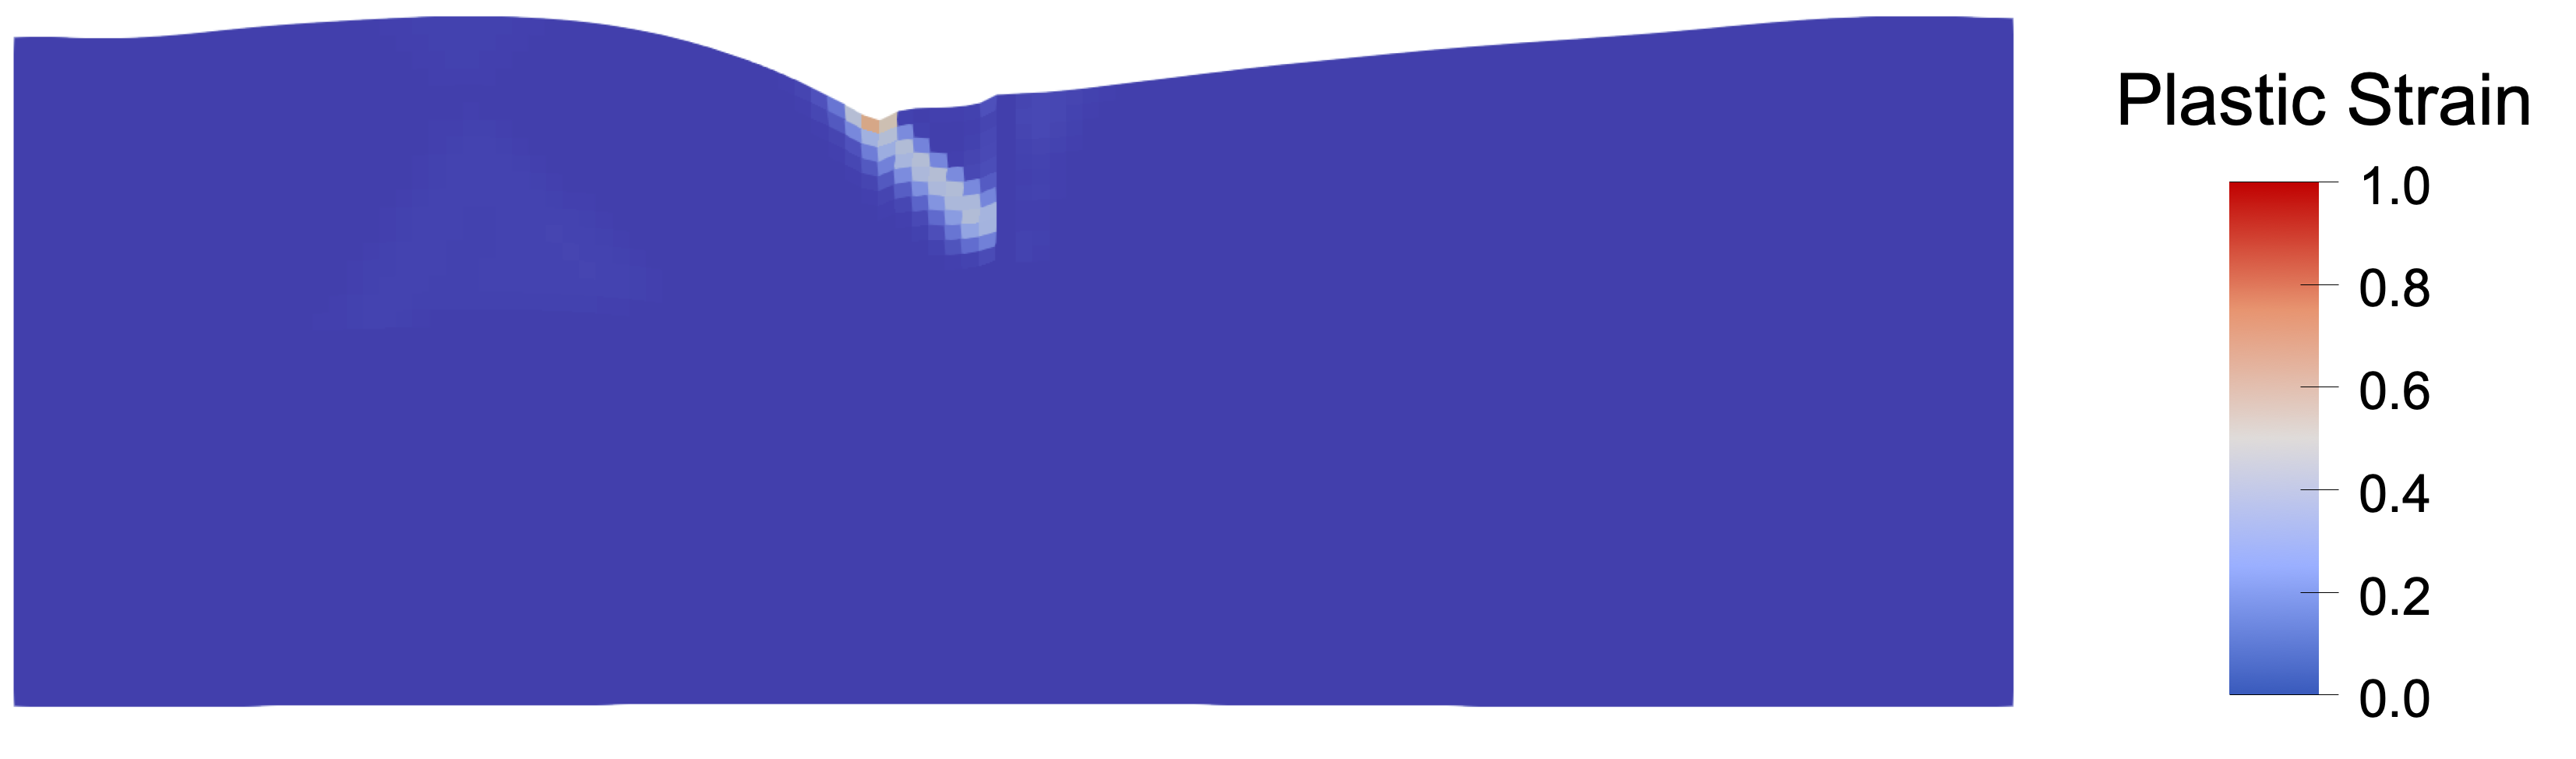
\includegraphics[width=0.9\linewidth]{./figs/kfault_m05.png}
	\caption{Snapshots of plastic strain distribution in the kinematic model with M = 0.5 over 1 Myr at 0.1 Myr interval. Bands of localized plastic strain represent faults.}
	\label{fig:kfault_m05}
\end{figure}
\begin{figure}[!htb]
	\centering
	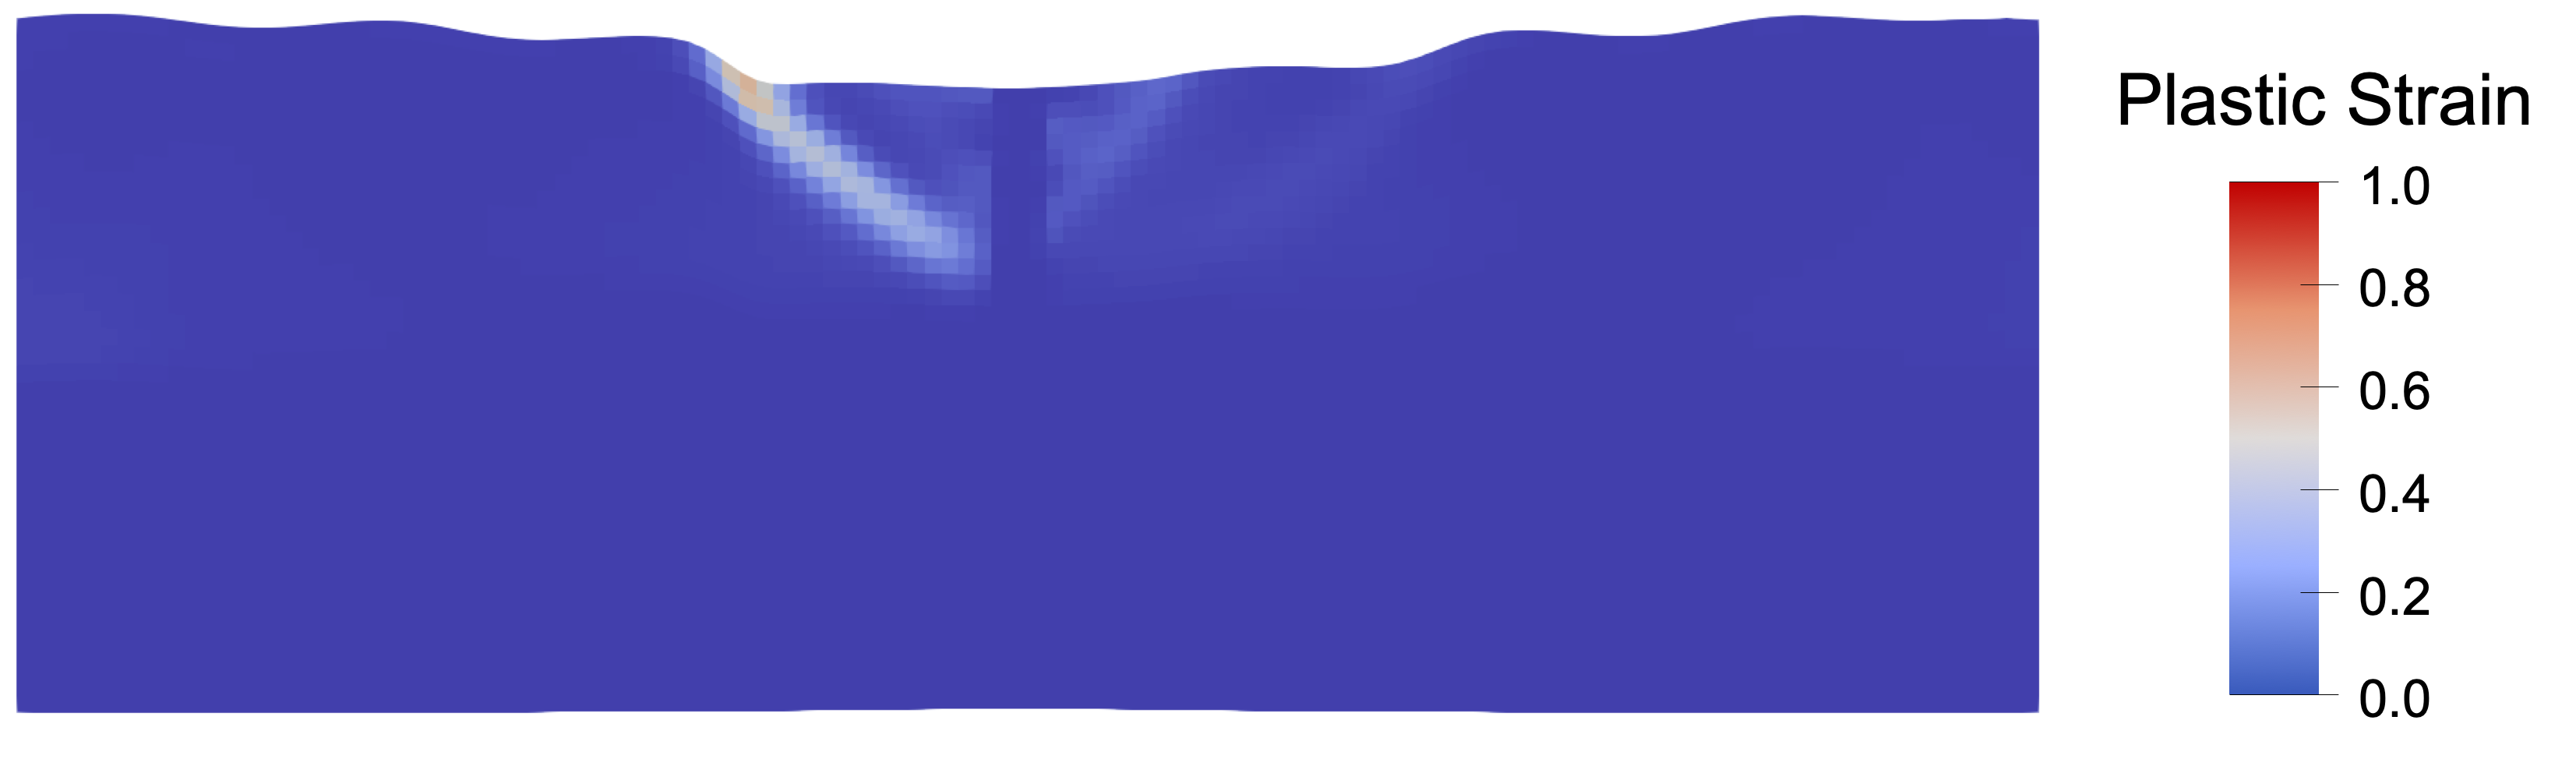
\includegraphics[width=0.9\linewidth]{./figs/kfault_m08.png}
	\caption{Same as Fig.~\ref{fig:kfault_m05} but from the kinematic model with M = 0.8.}
	\label{fig:kfault_m08}
\end{figure}

Mean horizontal velocity of each plate ($\overline{\boldsymbol{v}}_{x}$), x component of the nodal velocities averaged over the nodes on each side of the ridge axis, show different pattern depending on M values. in the kinematic models. When M = 0.5, $\overline{\boldsymbol{v}_x}$ remain constant at 2.5 cm/yr on right-side plate and 2.2 cm/yr on left-side plate (Figure \ref{fig:km05}). At M = 0.8, $\overline{\boldsymbol{v}_x}$ have two phases (Figure \ref{fig:km08}). For the first 190 Kyrs, the right-side plate is in a low-velocity phase while the left-side plate is in a high-velocity phase. From 190 to 330 Kyrs, now the right-side plate is in a high-velocity phase and the left-side plate is in a low-velocity phase. \note[EC]{I thought you would show the mean horizontal plate velocity plot after removng the remeshing signals. They are included in the current plots, right?} \note[HC]{The problem is that the filtered signal cannot represent the sharp edges. So I think not showing is better especially in kinematic and Fres=0 cases. I'll explain more of this in our meeting.} This pattern repeats until the model ends.

\begin{figure}[!htb]
	\centering
	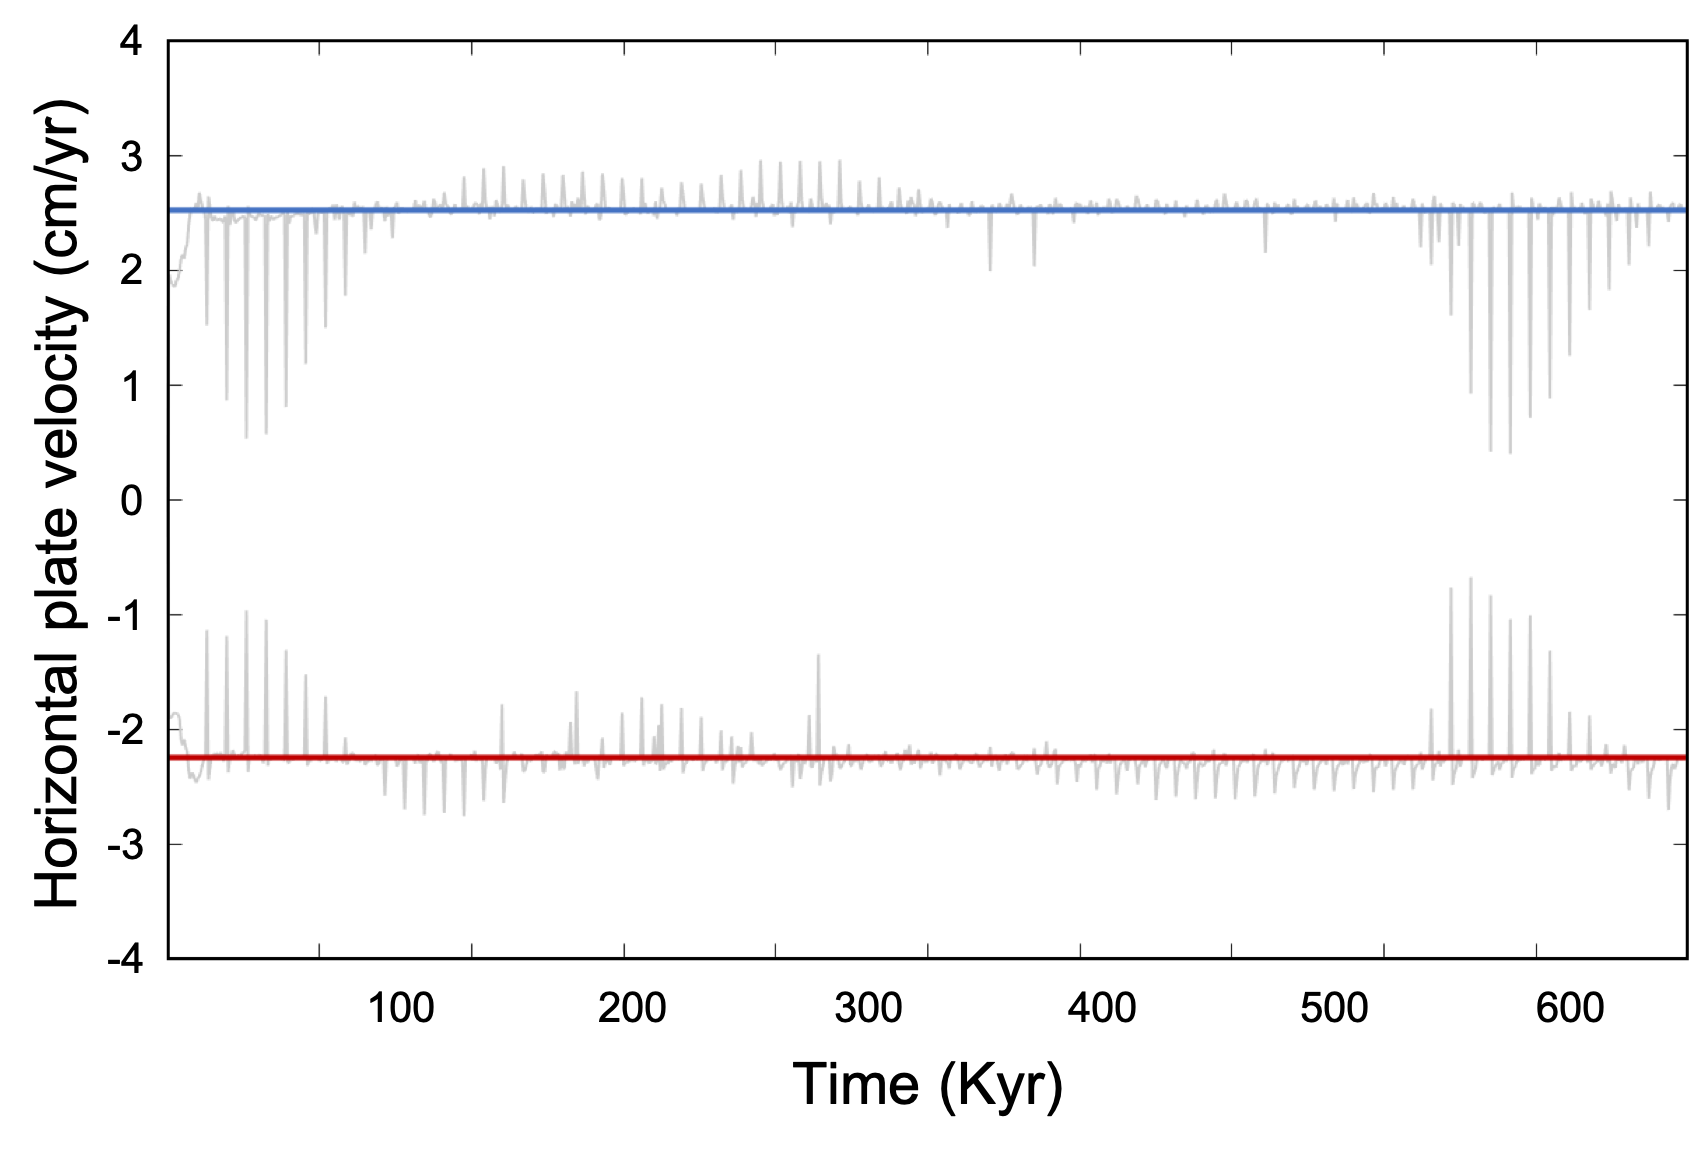
\includegraphics[width=0.9\linewidth]{./figs/km05.png}
	\caption{Mean horizontal plate velocities from the M=0.5 kinematic model. For reference, 2.5 cm/yr and $-$2.2 cm/yr are plotted as blue and red lines.}
	\label{fig:km05}
\end{figure}
\begin{figure}[!htb]
	\centering
	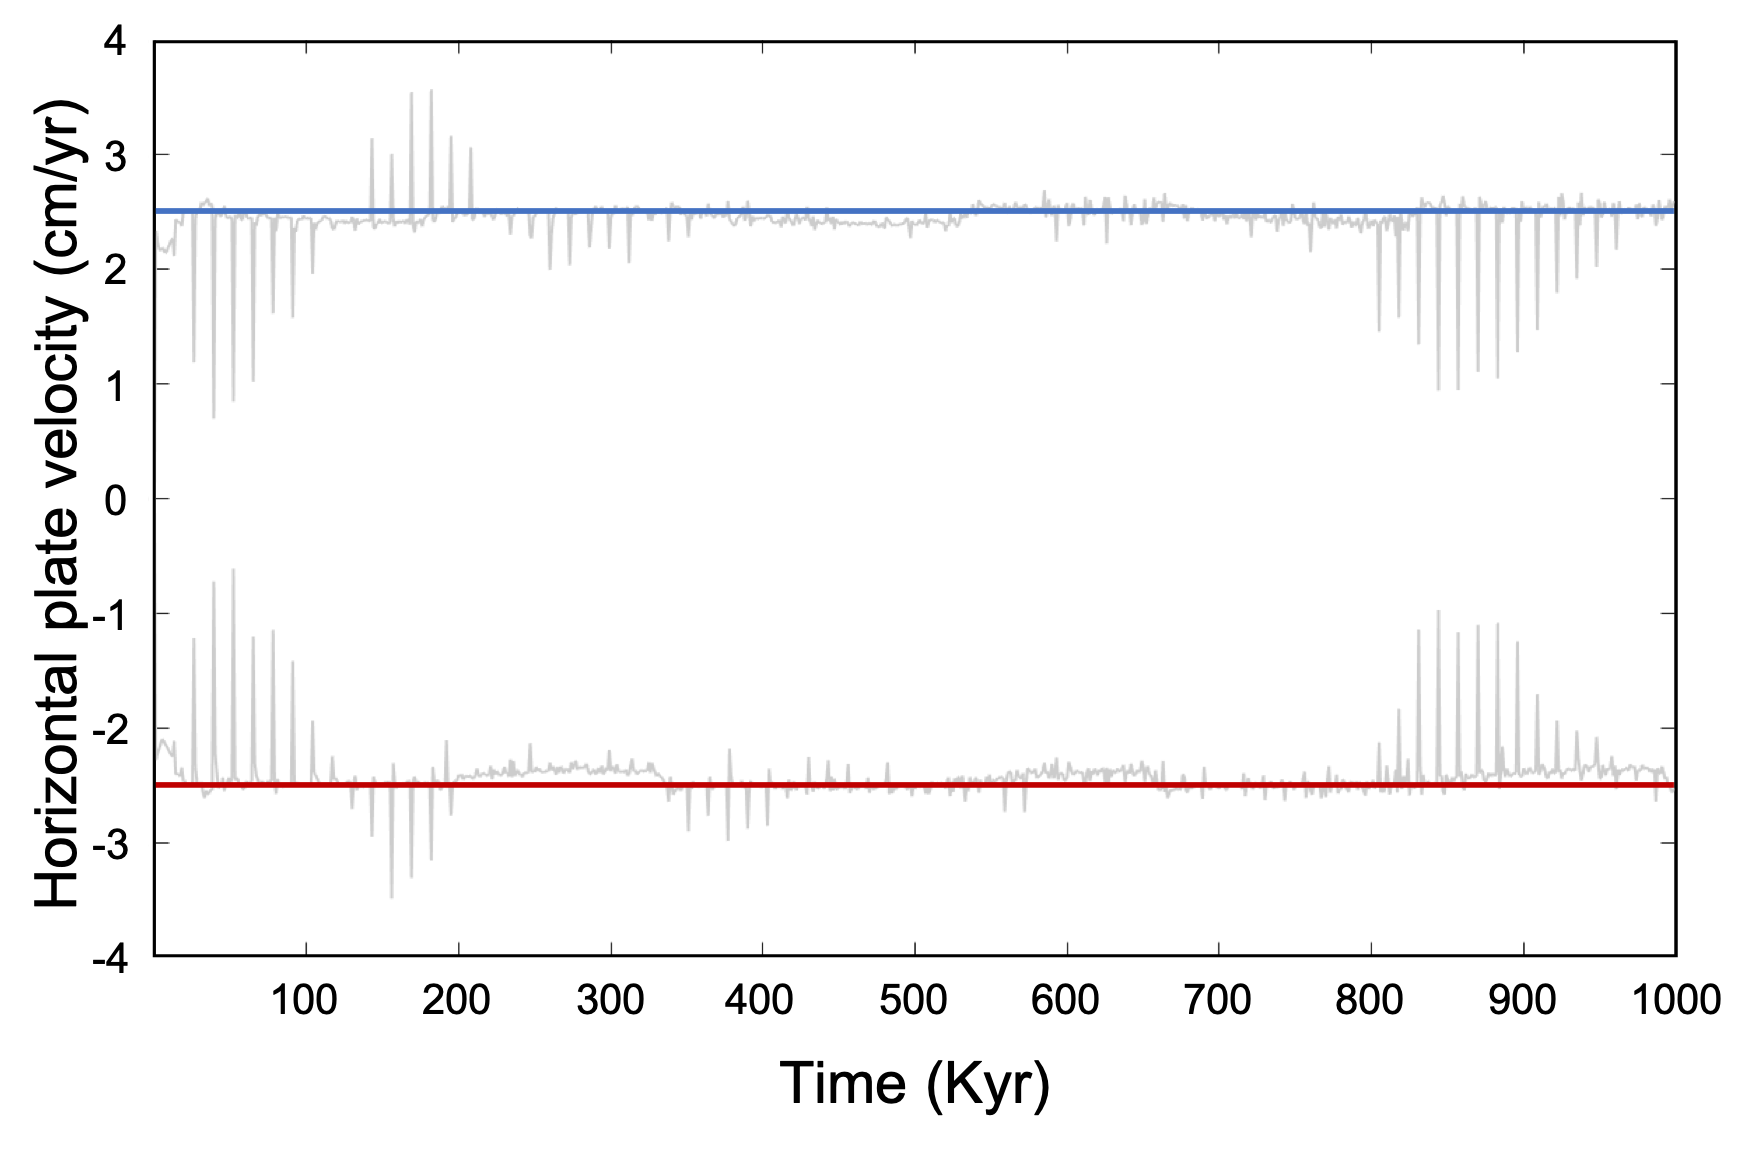
\includegraphics[width=0.9\linewidth]{./figs/km08.png}
	\caption{Mean horizontal plate velocity obtained from M=0.8 kinematic model. As a reference, 2.5 cm/yr and $-$2.5 cm/yr are plotted as blue and red lines.}
	\label{fig:km08}
\end{figure}
\begin{figure}[!htb]
	\centering
	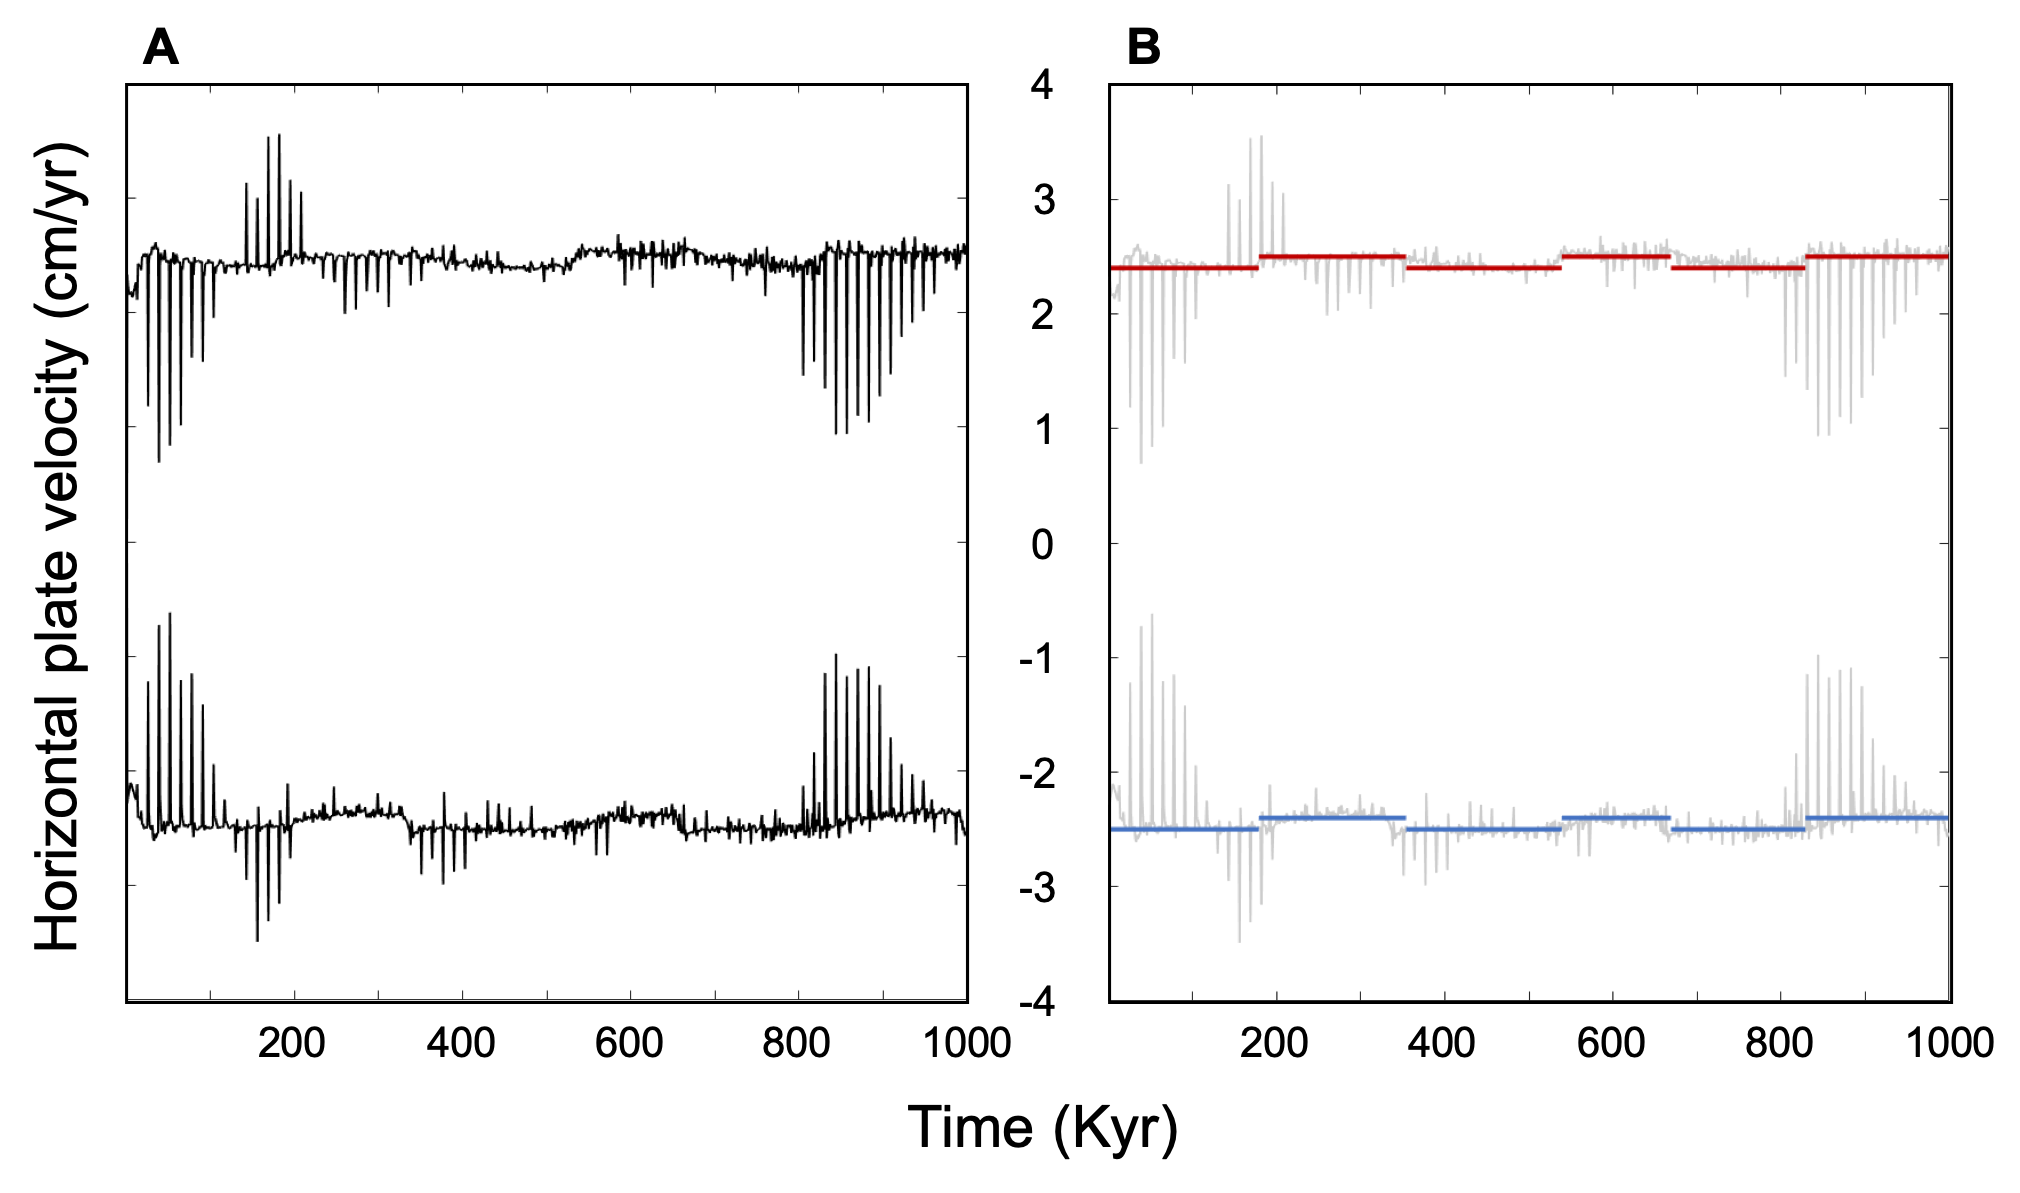
\includegraphics[width=0.95\linewidth]{./figs/kinm08.png}
	\caption{\textbf{A.} Raw mean horizontal plate velocity from M=0.8 kinematic model. \textbf{B.} Mean horizontal plate velocity after removing the remeshing effects. The red and blue lines are the picked mean horizontal plate velocity. \note[HC]{How about this way?}}
	\label{fig:kinm08}
\end{figure}
%However, the velocity-driven models do not show the observed non-uniform plate velocity by simply changing magmatism at the spreading center.


\section{$(\boldsymbol{F_{res}})_x=0$ models}

This condition represents the hypothetical state where $\boldsymbol{F}_{bdy}$ is adjusted such that it perfectly counteracts $\boldsymbol{F}_{int}$ making $\boldsymbol{F}_{res}$ equal to zero all the time. Since the net residual force is zero on the side boundaries, the models under this condition show constant plate velocity as expected for a motion with zero acceleration.

\subsection{Constant M models}

With this force boundary condition and fixed M value, models mimic the appearance of the constant velocity boundary condition models (Figure \ref{fig:force0}). Models produce one master detachment fault when M = 0.5 (Figure \ref{fig:f0fault}A) and series of small offset normal faults when M = 0.8(Figure \ref{fig:f0fault}A).
%
\begin{figure}[!htb]
	\centering
	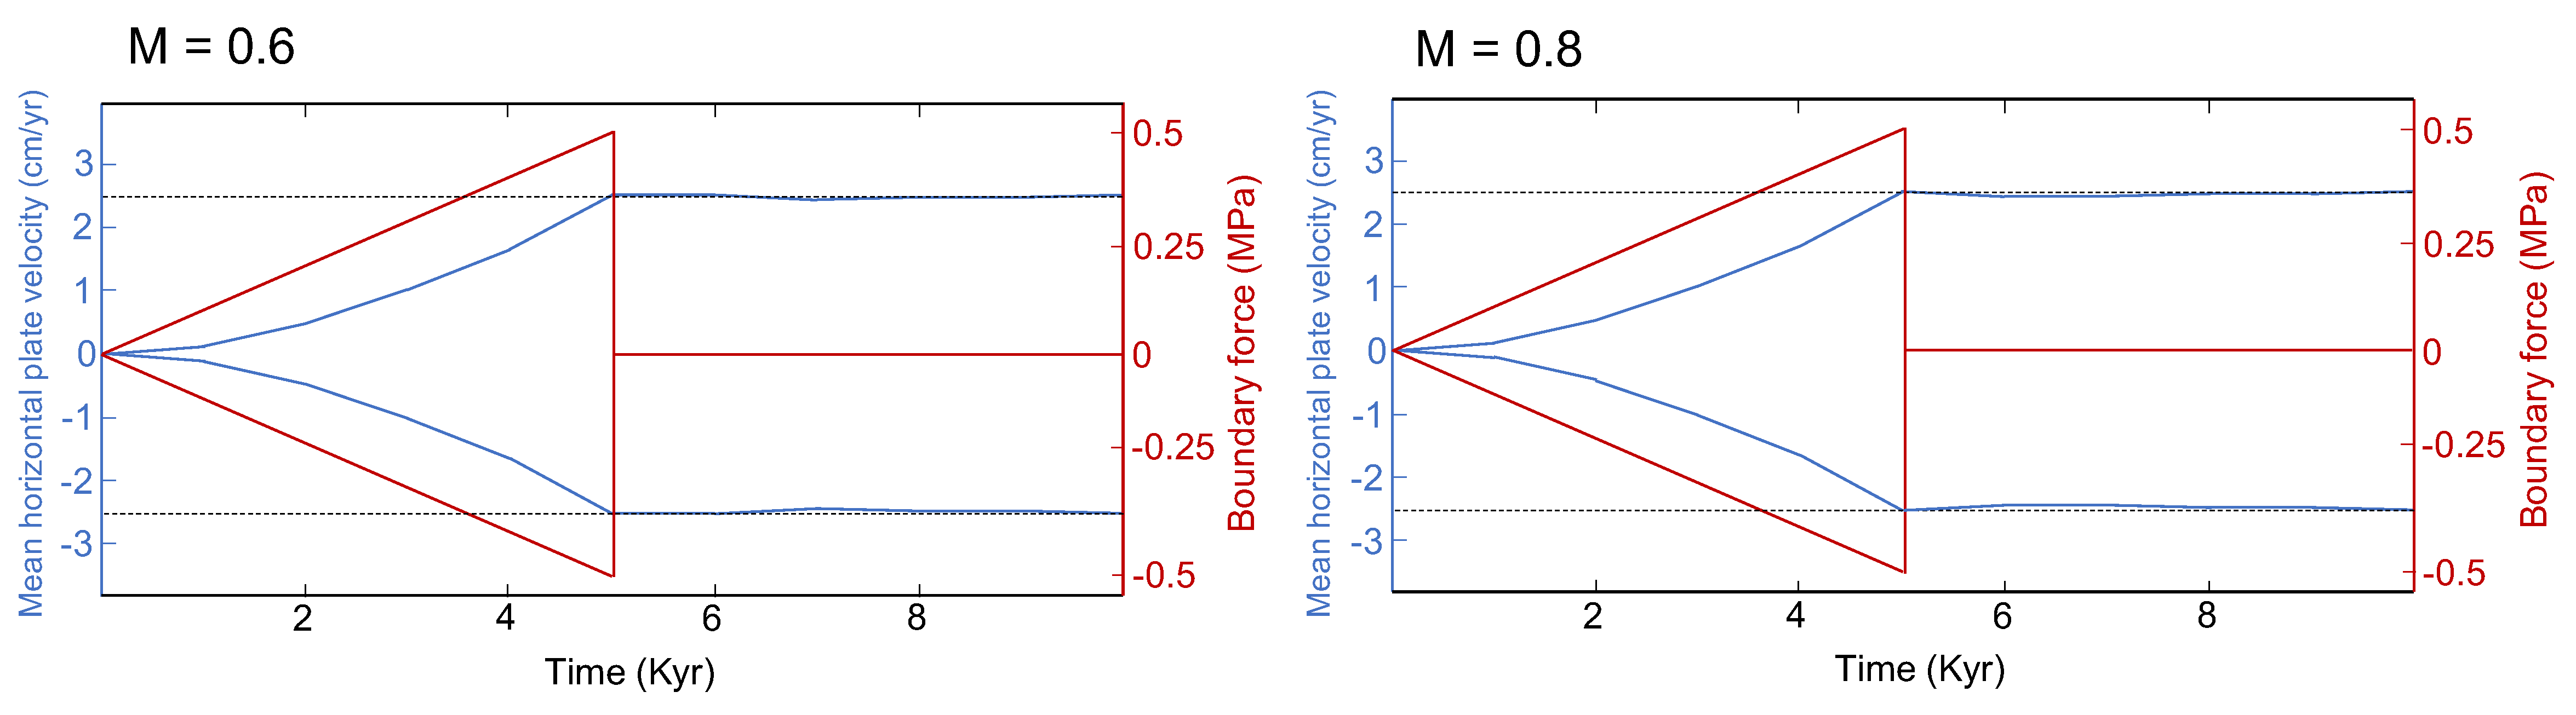
\includegraphics[width=0.99\linewidth]{./figs/force0.pdf}
	\caption{Velocity and boundary force($(\boldsymbol{F_{bdy}})_x$) as a function of time. $(\boldsymbol{F_{bdy}})_x$ increases linearly with time until the plate speed quadratically increase to 2.5 cm /yr. At that moment, $(\boldsymbol{F_{bdy}})_x$ is reduced to zero so that the horizontal plate velocity is maintained at the target value of 2.5 cm/yr.}
	\label{fig:force0}
\end{figure}
\begin{figure}[!htb]
	\centering
	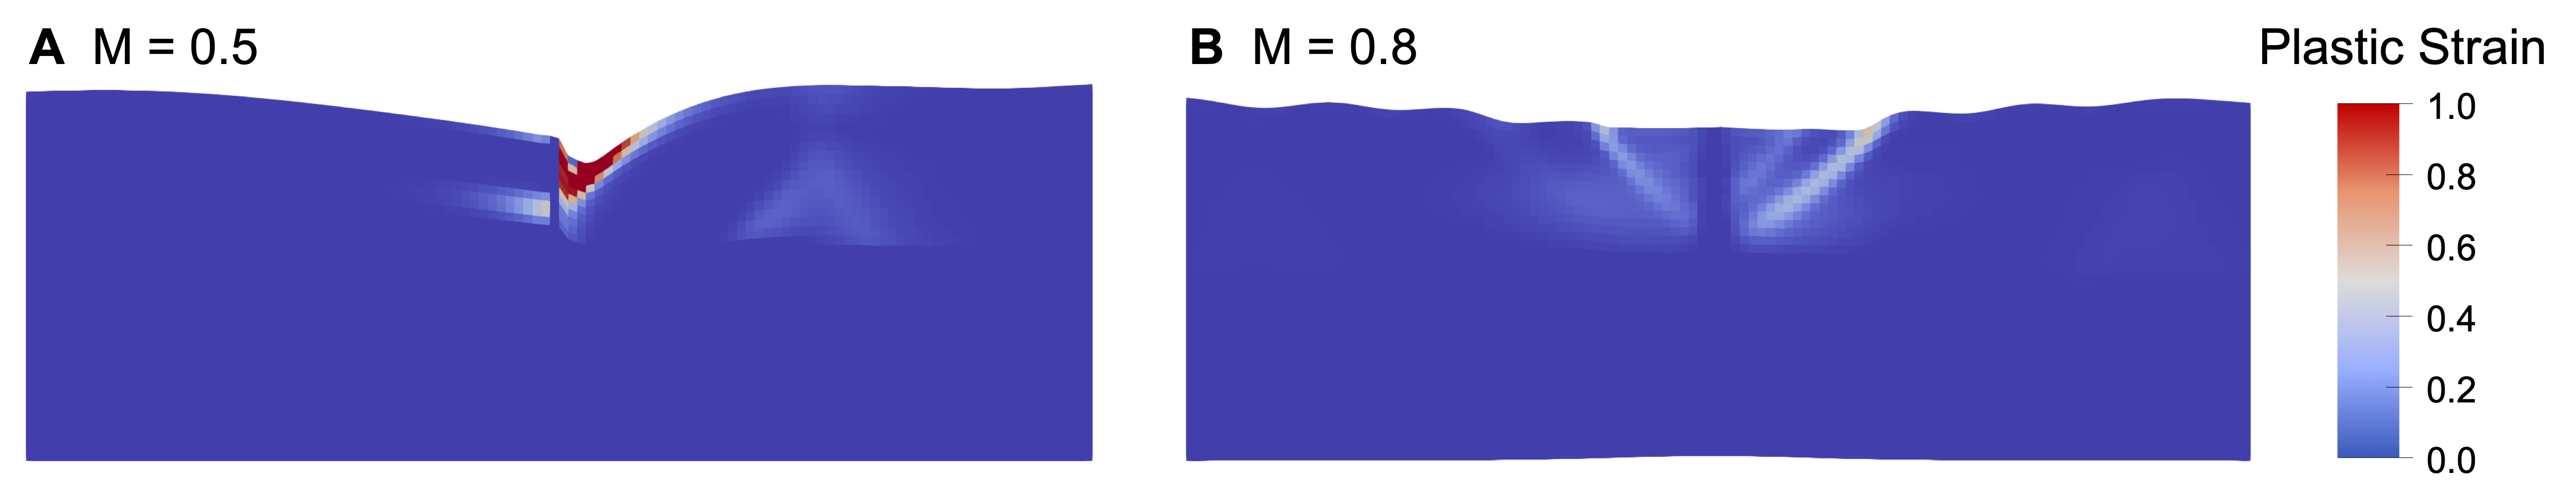
\includegraphics[width=0.99\linewidth]{./figs/f0fault.png}
	\caption{\textbf{A.} Snapshots of fault behavior of the $(\boldsymbol{F_{res}})_x=0$ model for M = 0.5 after 1Myr. Model shows detachment faulting. \textbf{B.} Same as \textbf{A} but for M = 0.8. Model shows alternating faulting.}
	\label{fig:f0fault}
\end{figure}

The models with $(\boldsymbol{F_{res}})_x=0$ condition show uniform horizontal plate velocity. At M = 0.5, plate velocities remain constant at 2.5 cm/yr on the right-side plate and 2.7 cm/yr on the left-side plate (Figure \ref{fig:f0vel}A). When M = 0.8, plate velocities have two phases (Figure \ref{fig:f0vel}B). For the first 280 Kyrs, the right-side plate is in a high-velocity phase while the left-side plate is in a low-velocity phase. From 280 to 420 Kyrs, now the right-side plate is in a low-velocity phase and the left-side plate is in a high-velocity phase. This pattern repeats until the model ends.

\begin{figure}[!htb]
	\centering
	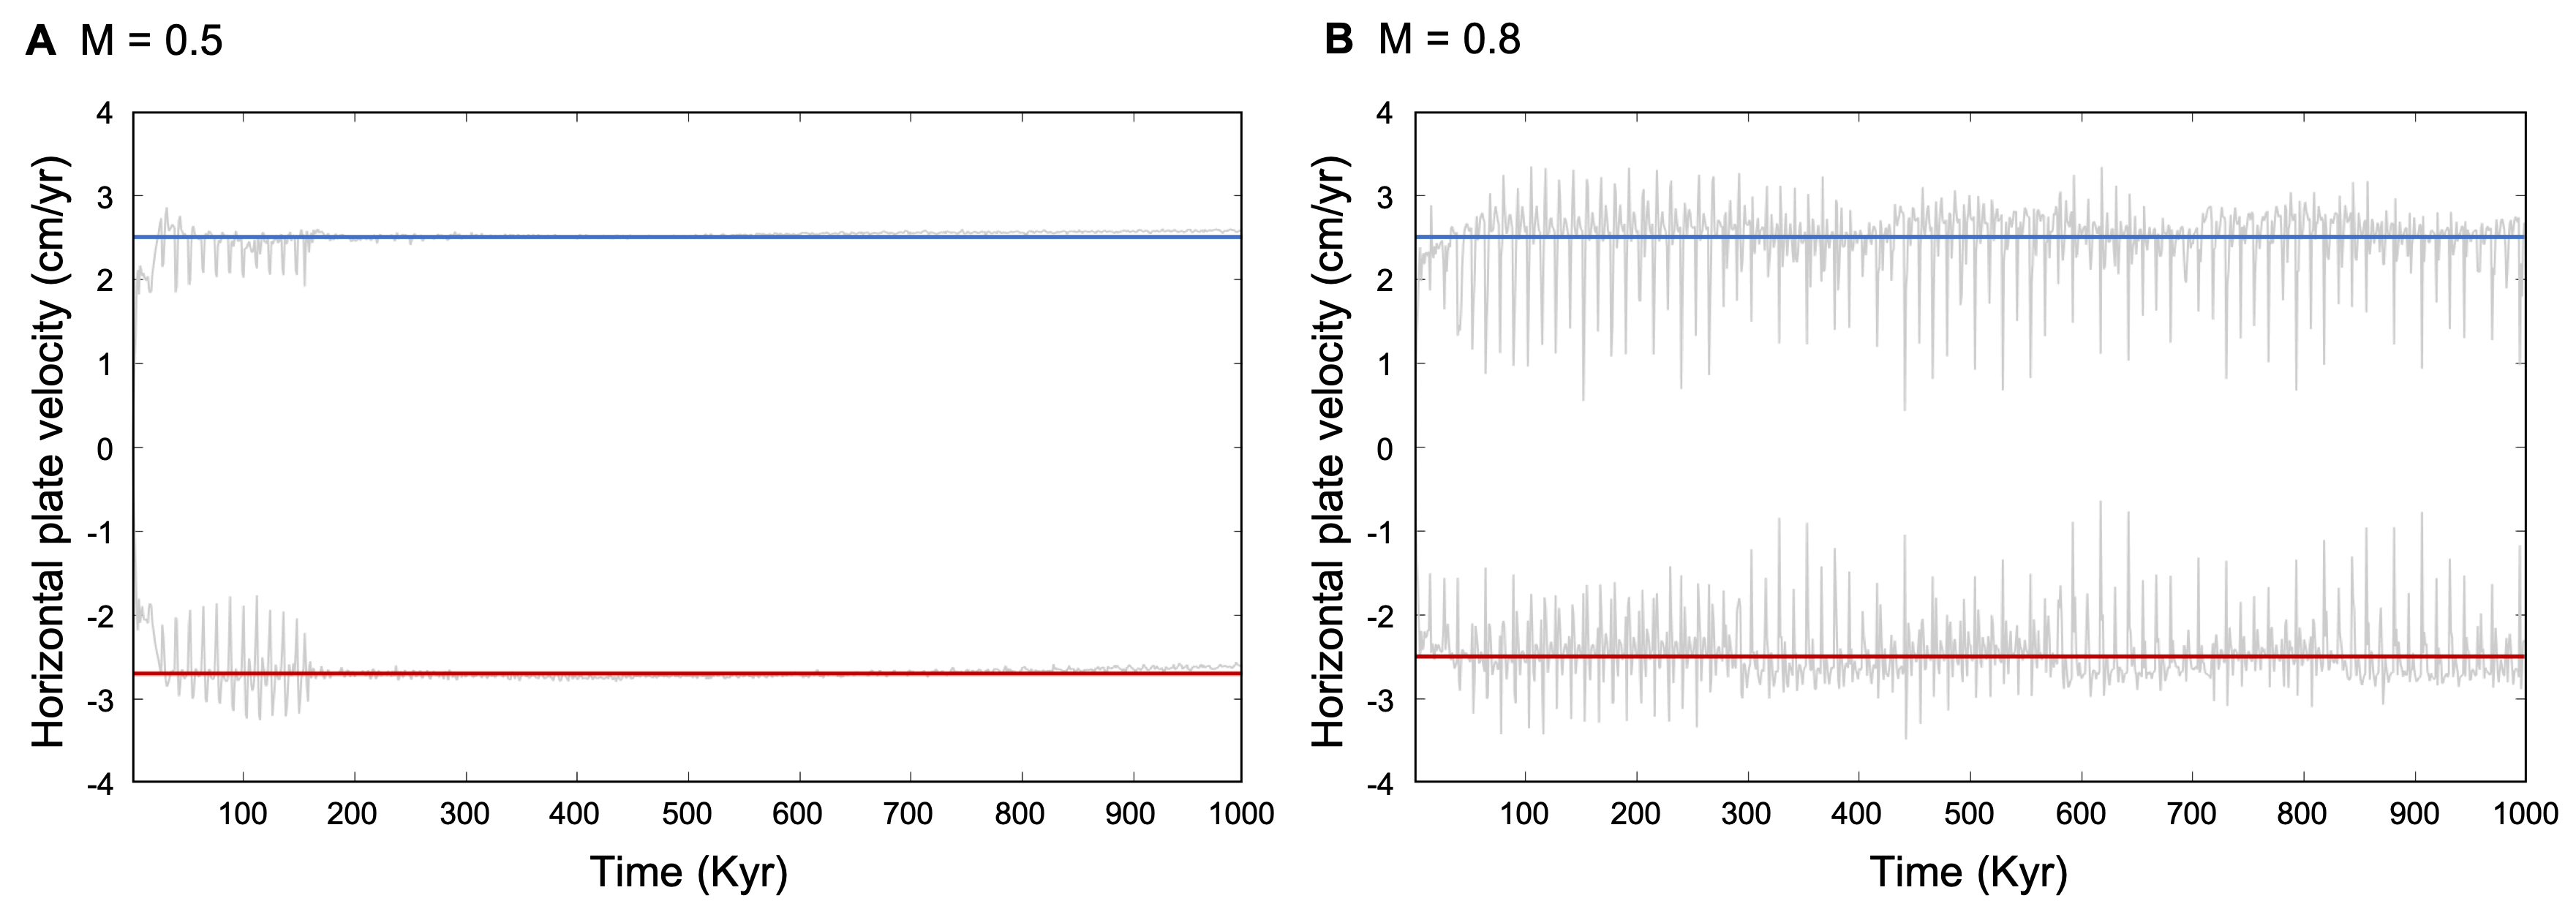
\includegraphics[width=0.99\linewidth]{./figs/f0vel.png}
	\caption{\textbf{A.} Horizontal plate velocity obtained from M=0.5 $(\boldsymbol{F_{res}})_x=0$ model results. As a reference, 2.5 cm/yr and $-$2.7 cm/yr are plotted as blue and red lines. \textbf{B.} Same as \textbf{A} but for M = 0.8. As a reference, 2.5 cm/yr and $-$2.5 cm/yr are plotted as blue and red lines.}
	\label{fig:f0vel}
\end{figure}

\subsection{Time-variable M models}

Changing M value over time means the ratio of magmatic accretion rate to total plate spreading rate changes over time. In order to investigate how magmatism at spreading center affects the velocity of the plate, I test two time-variable M models, from M = 0.5 to 0.8 after 400 Myrs and vice versa. The case of magmatic accretion increasing is represented by the model changing from M = 0.5 to 0.8, while decreasing magmatic accretion corresponds to the model with M = 0.8 to 0.5.

Two-phase M history models show expected faulting modes. When the model is in the phase of M = 0.5, it forms a master detachment fault on one side of the plate; and the model produces a symmetric pattern of small-offset faults when M = 0.8.

\begin{figure}[!htb]
	\centering
	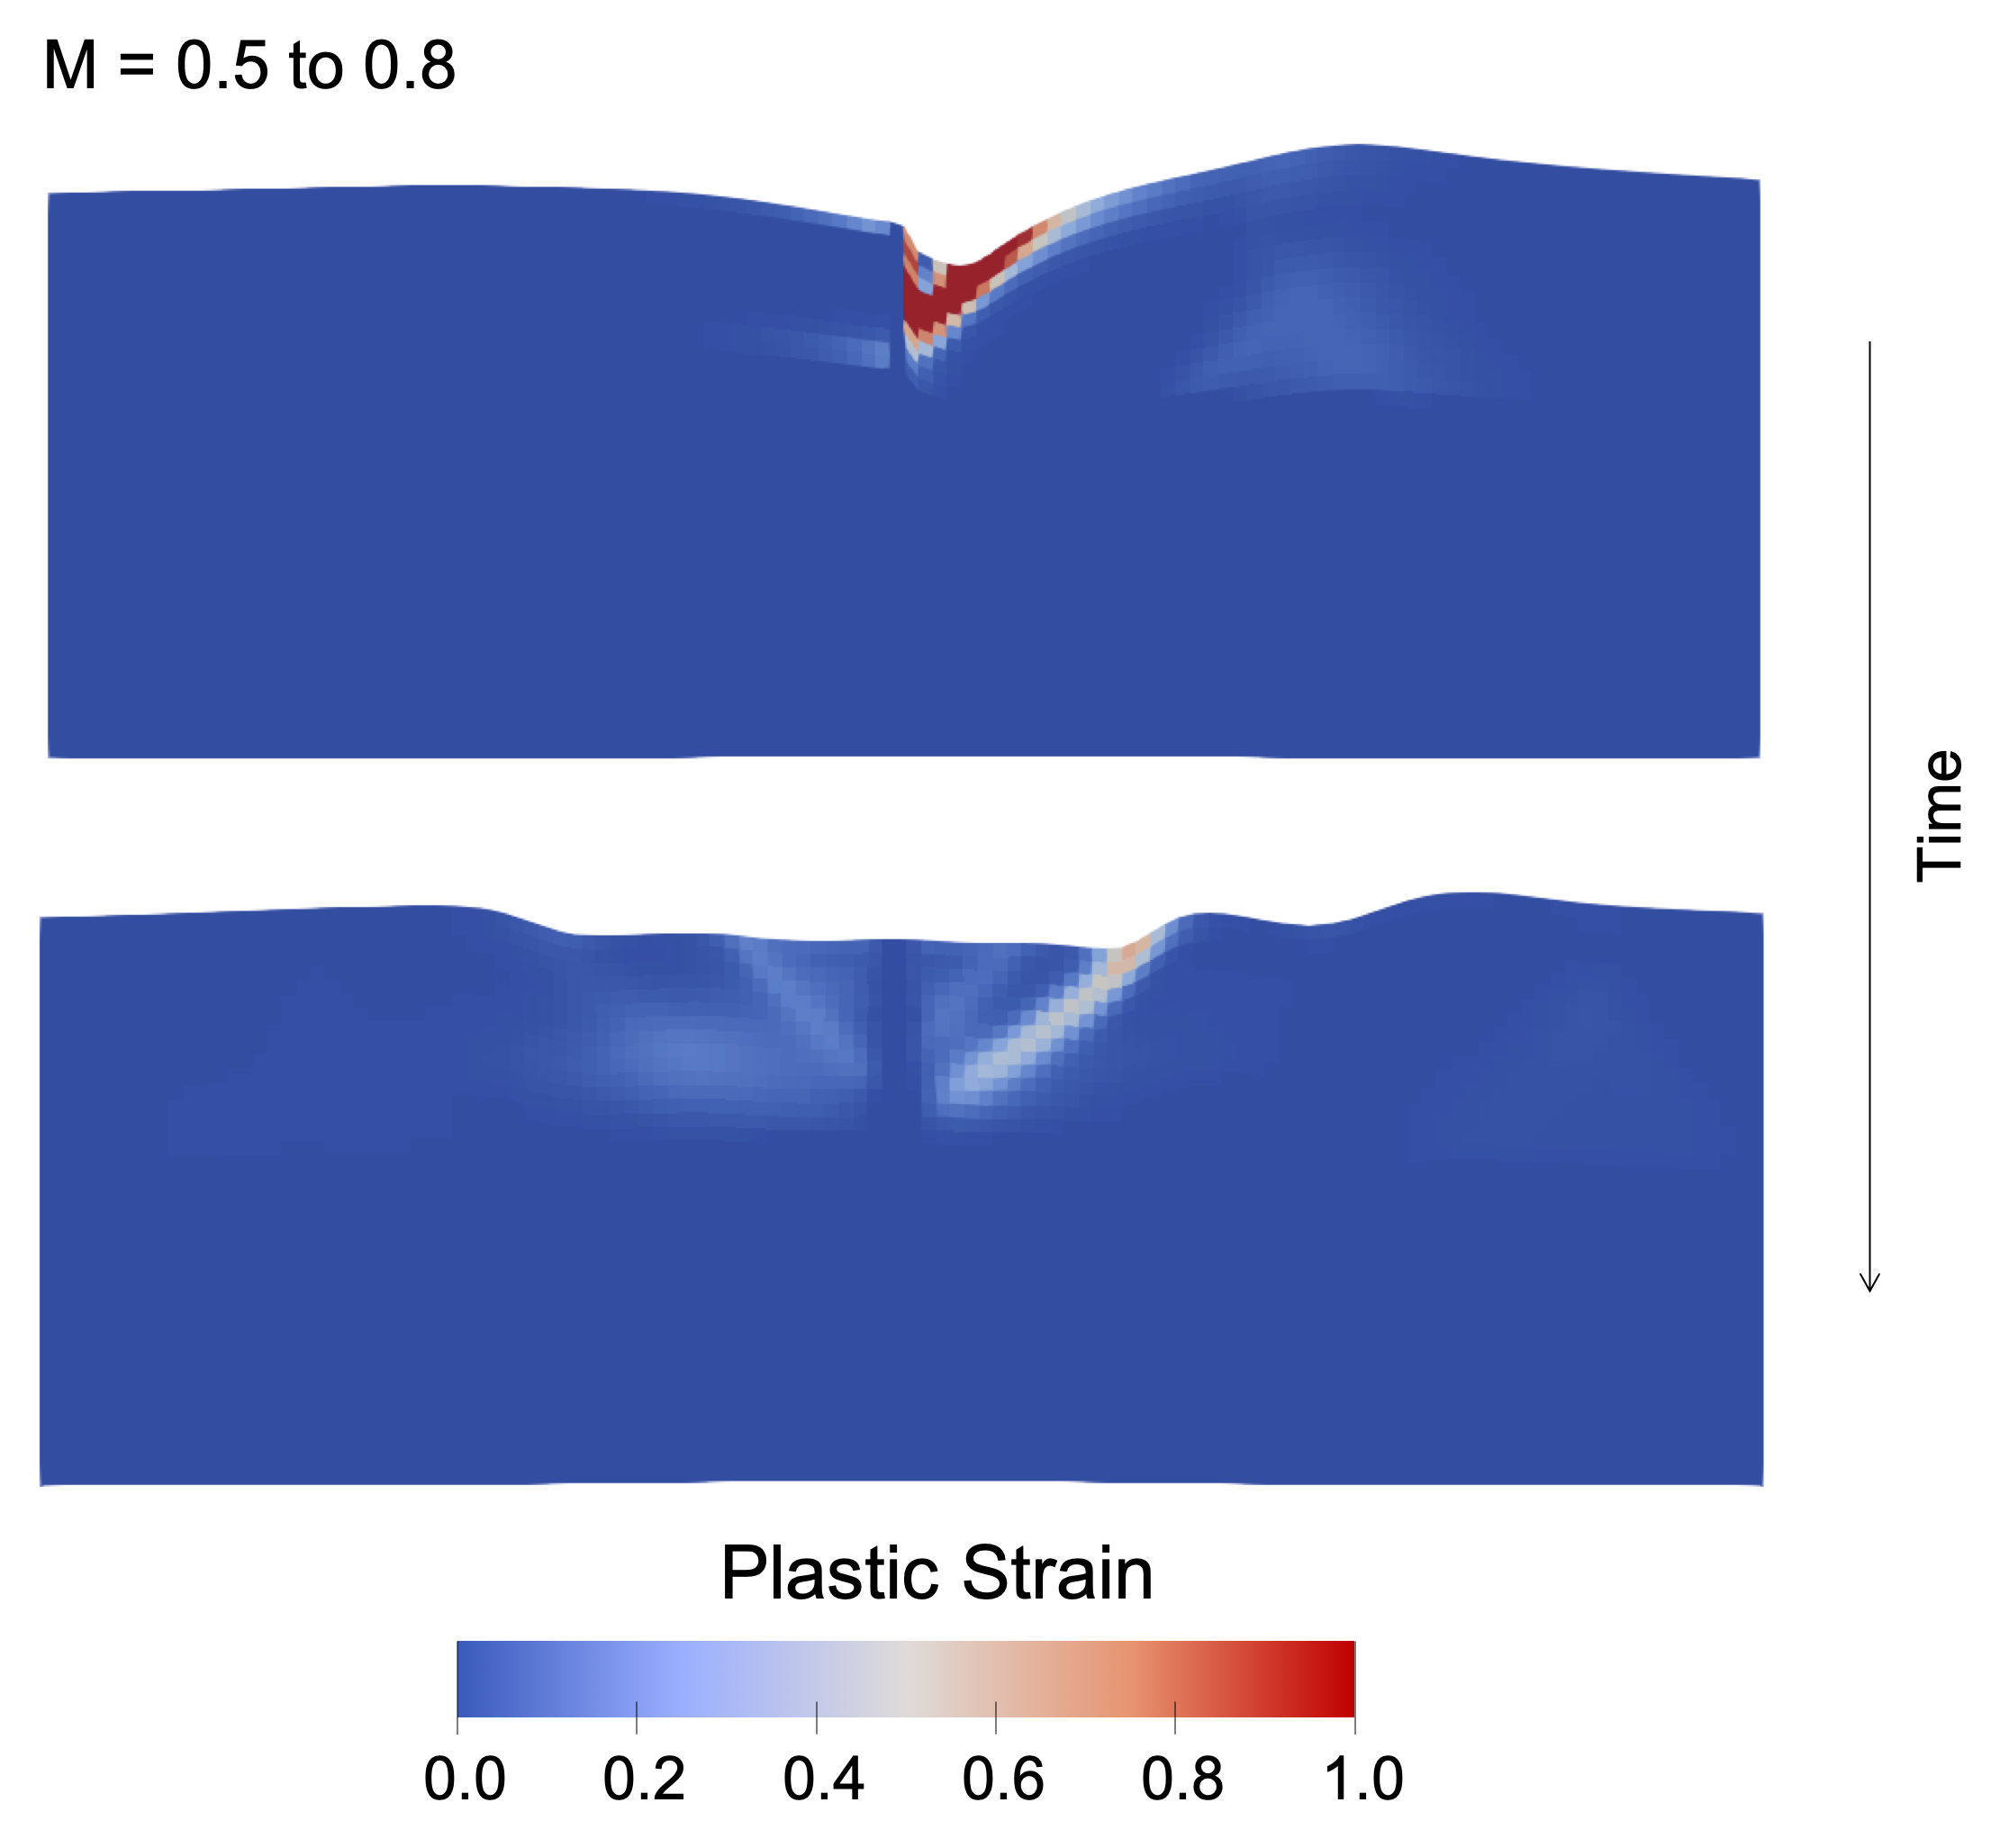
\includegraphics[width=0.8\linewidth]{./figs/f0faultm05to08.png}
	\caption{Snapshots of fault behavior of the $(\boldsymbol{F_{res}})_x=0$ model for M = 0.5 to 0.8 after 400 Kyrs and 1Myr later. Model shows detachment faulting mode at initial stage but alternating faulting mode after changing M to 0.8.}
	\label{fig:f0fault05to08}
\end{figure}
\begin{figure}[!htb]
	\centering
	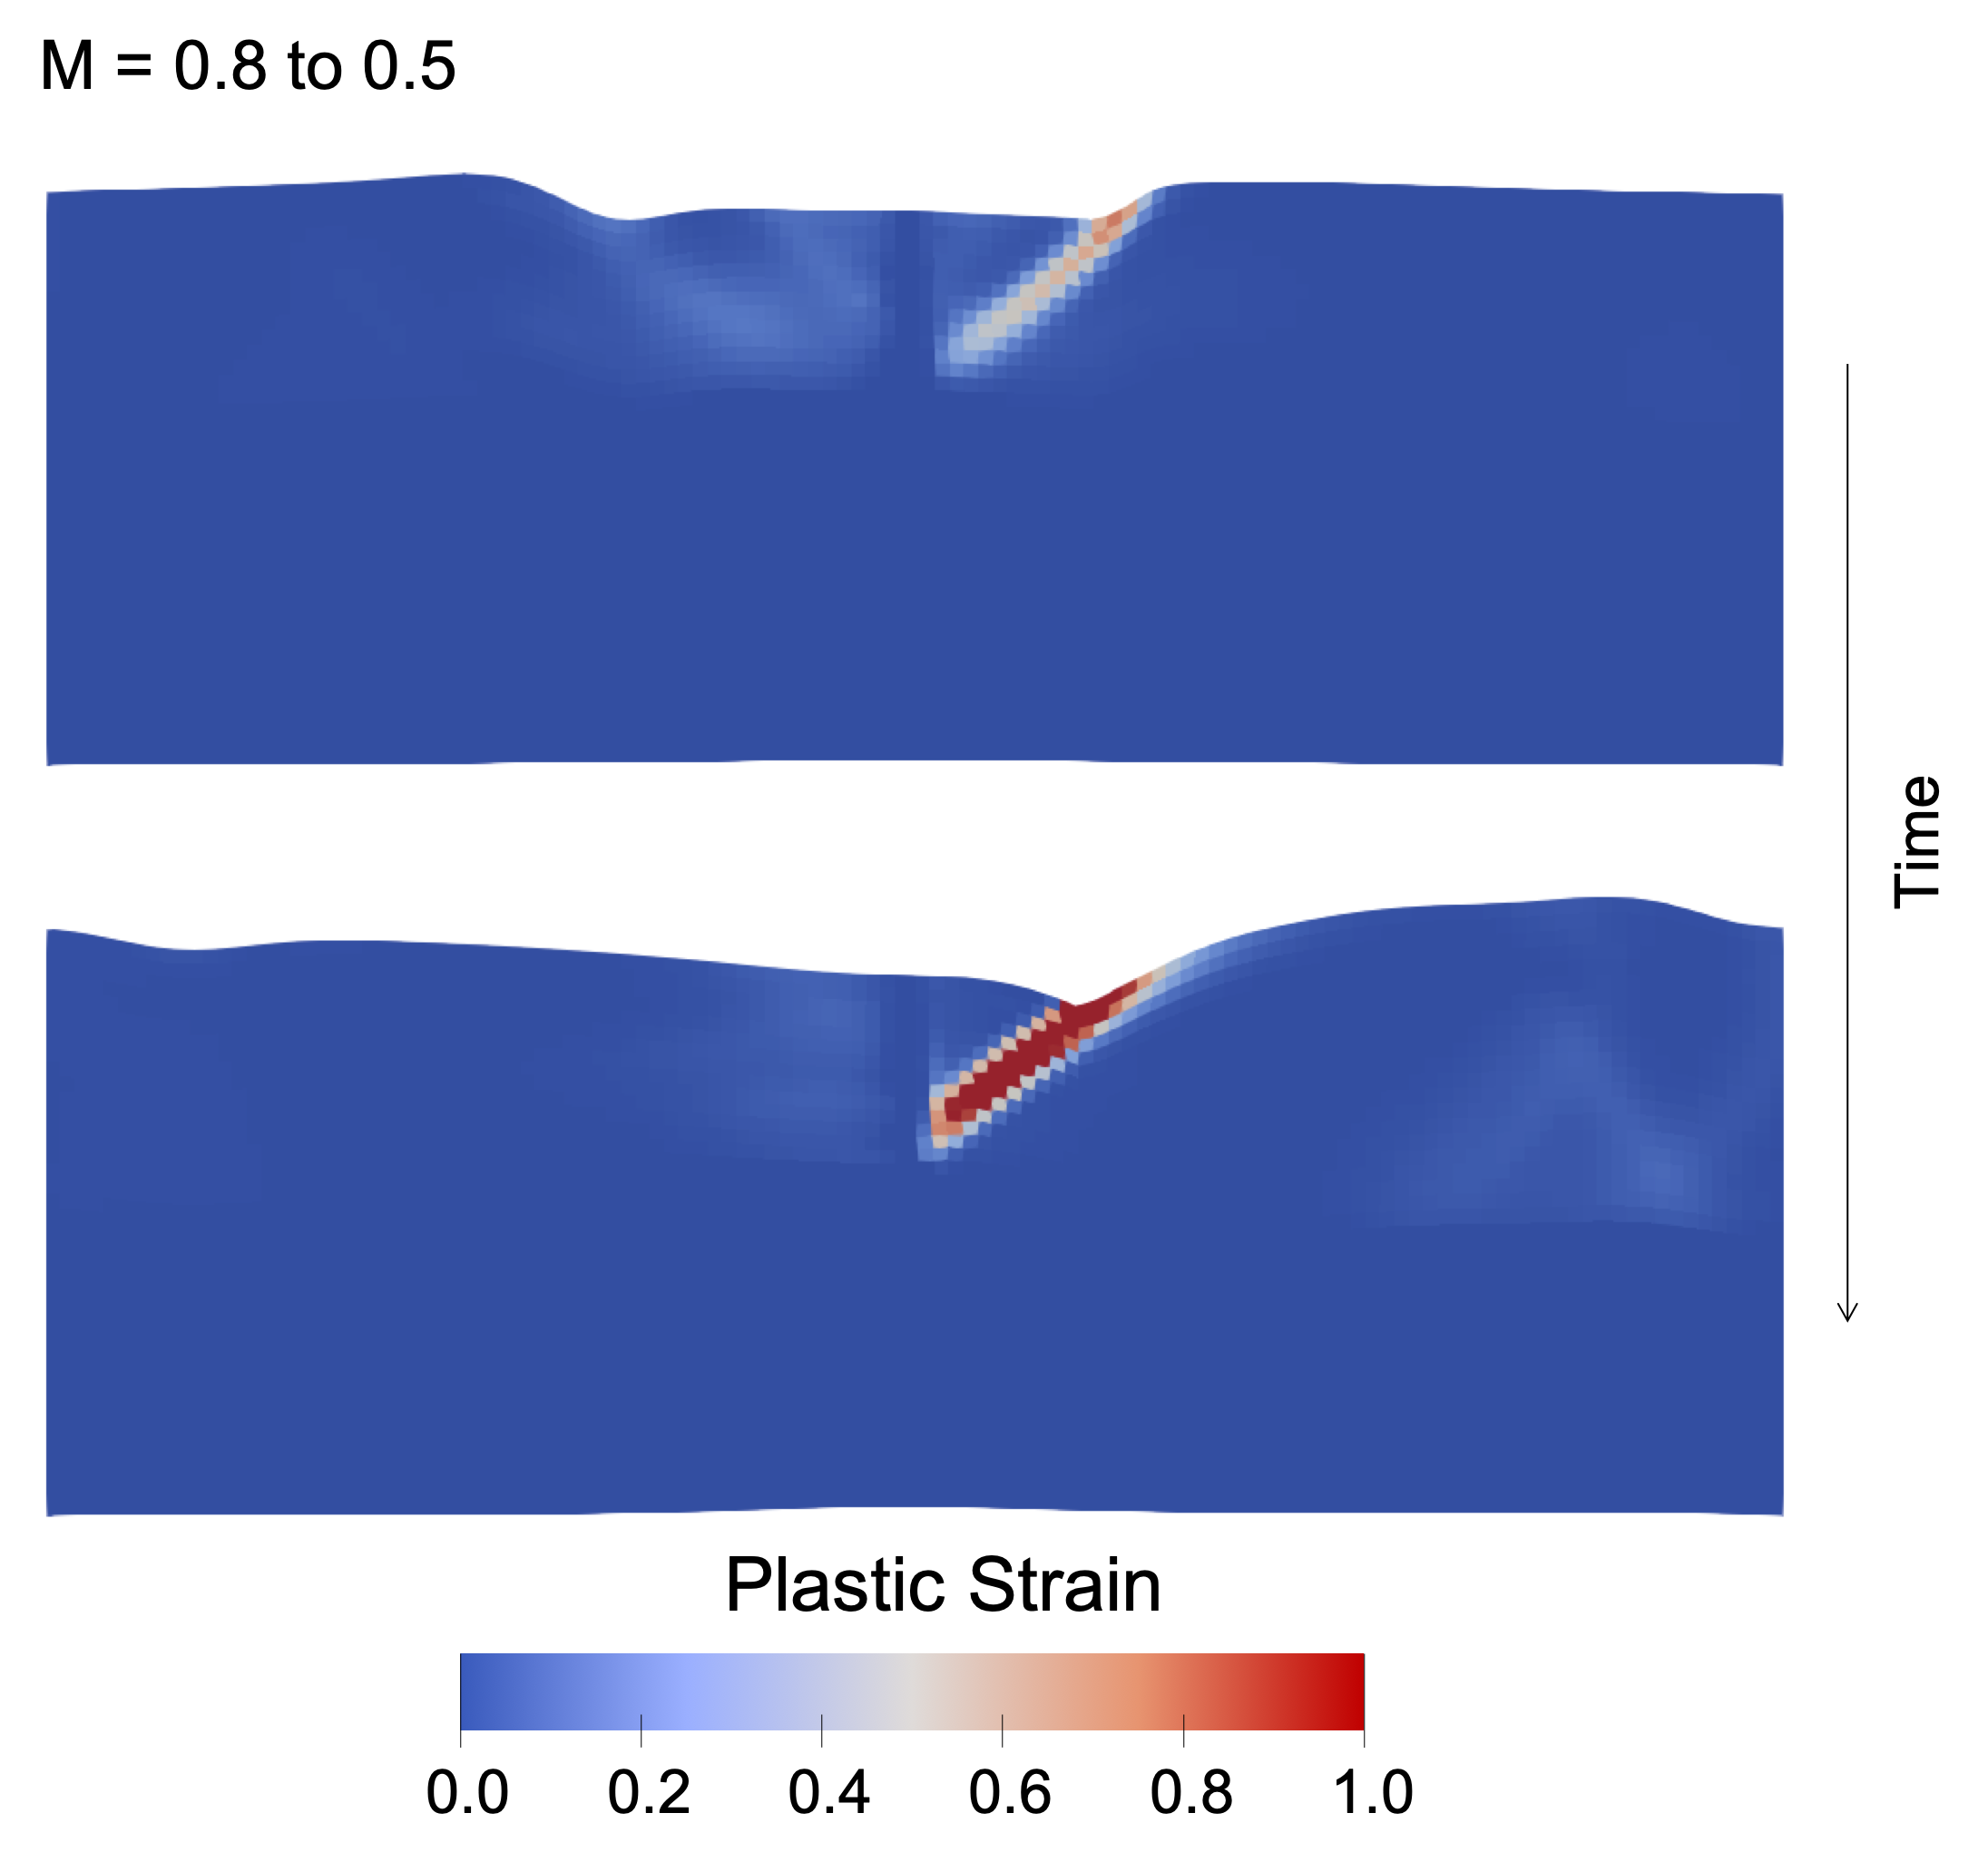
\includegraphics[width=0.8\linewidth]{./figs/f0faultm08to05.png}
	\caption{Snapshots of fault behavior of the $(\boldsymbol{F_{res}})_x=0$ model for M = 0.8 to 0.5 after 400 Kyrs and 1Myr later. Initially model shows alternating faulting mode but after changing M to 0.8, alternating faulting mode is visible.}
	\label{fig:f0fault05to08}
\end{figure}

The horizontal plate velocity changes when M value changes (400 Kyrs later). In M = 0.5 to 0.8 case, the right-side plate velocity remains constant at 2.5 cm/yr; and the left-side plate velocity remains constant at 2.7 cm/yr until 400 Kyrs. After changing M value to 0.8, two-phased velocity is visible due to the alternating faulting mode. From 400 to 570 Kyrs, the right-side plate is in a high-velocity phase while the left-side plate is in a low-velocity phase. From 570 to 700 Kyrs, the right-side plate starts to be in a low-velocity phase and the left-side plate is in a high-velocity phase. This pattern repeats until the model ends (Figure \ref{fig:f005to08}). In the case of M = 0.8 to 0.5, the horizontal plate velocity follows M = 0.8 model at initial stage. After changing M value to 0.5, the left-side plate velocity becomes constant at 2.7 cm/yr and the right-side plate velocity becomes constant at 2.3 cm/yr (Figure \ref{fig:f008to05}).

\begin{figure}[!htb]
	\centering
	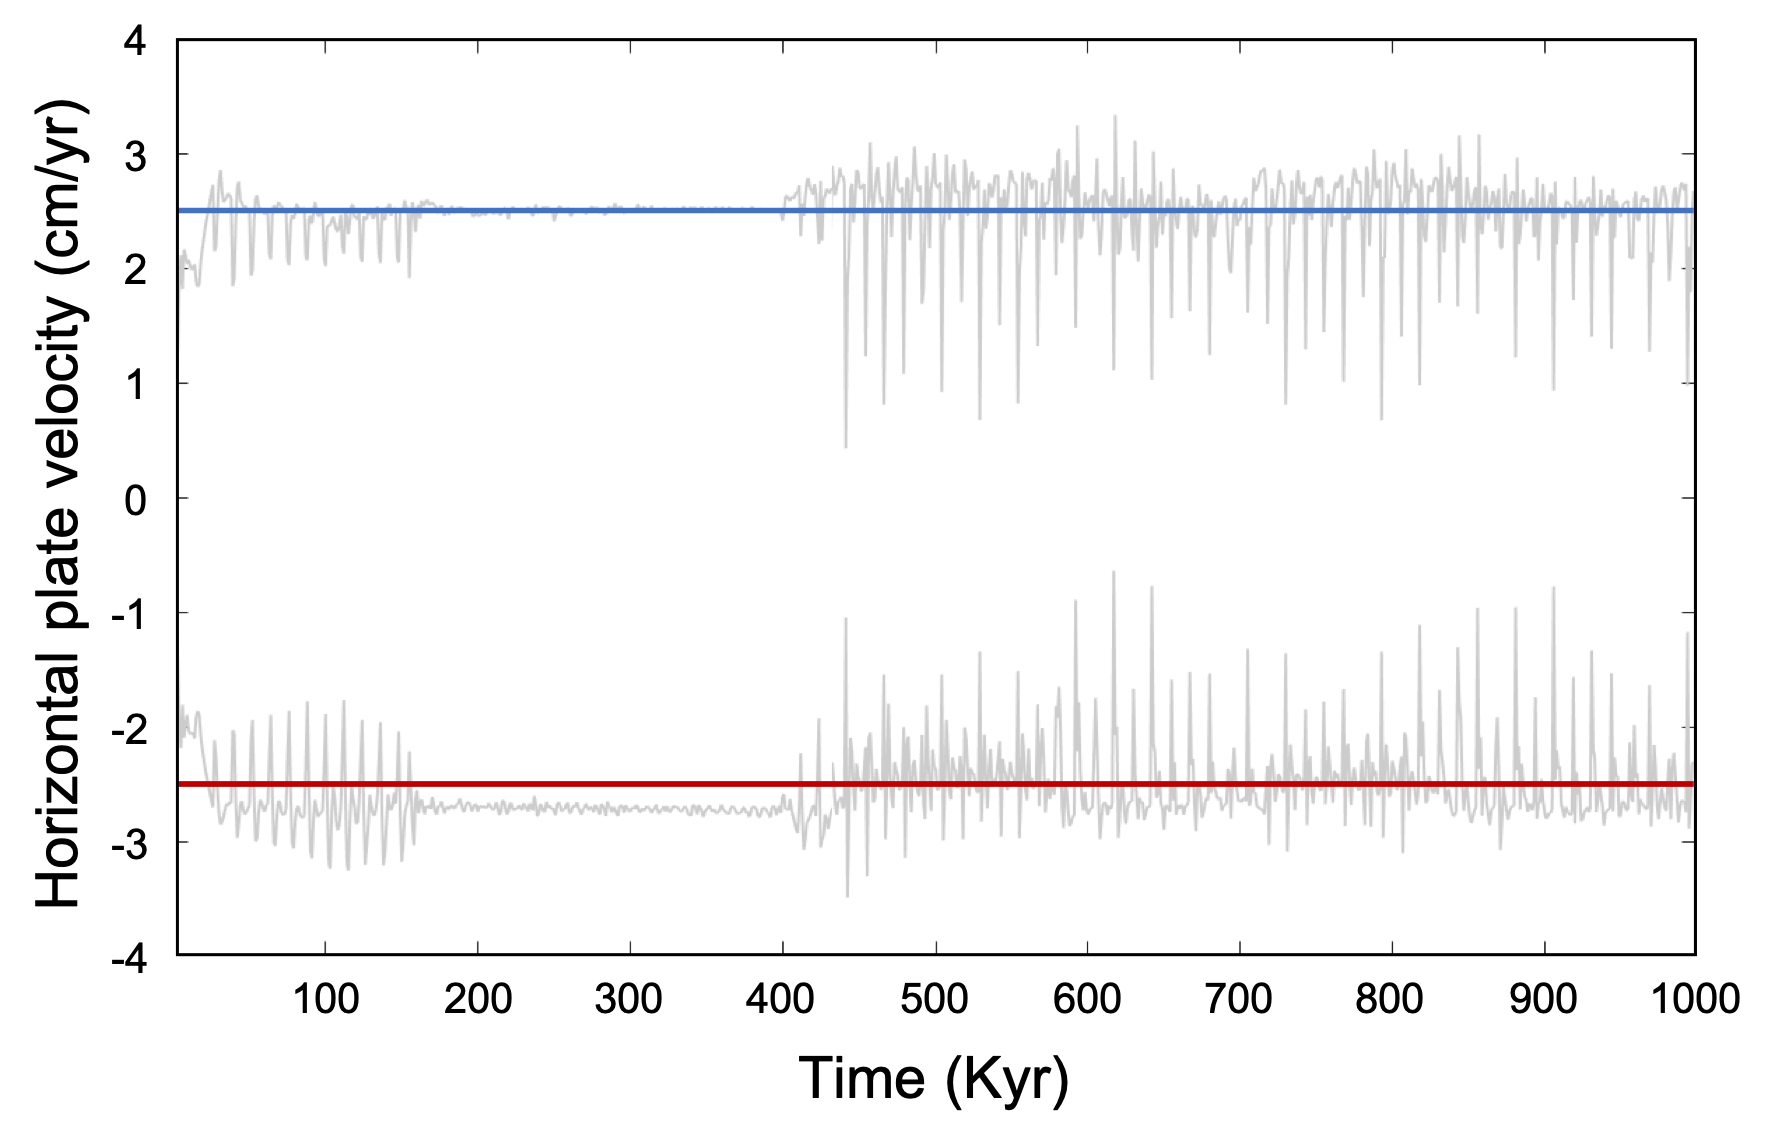
\includegraphics[width=0.9\linewidth]{./figs/f0m05to08.png}
	\caption{Horizontal plate velocity obtained from M=0.5 to 0.8 $(\boldsymbol{F_{res}})_x=0$ model. As a reference, 2.5 cm/yr and -2.5 cm/yr are plotted as blue and red lines.}
	\label{fig:f005to08}
\end{figure}
\begin{figure}[!htb]
	\centering
	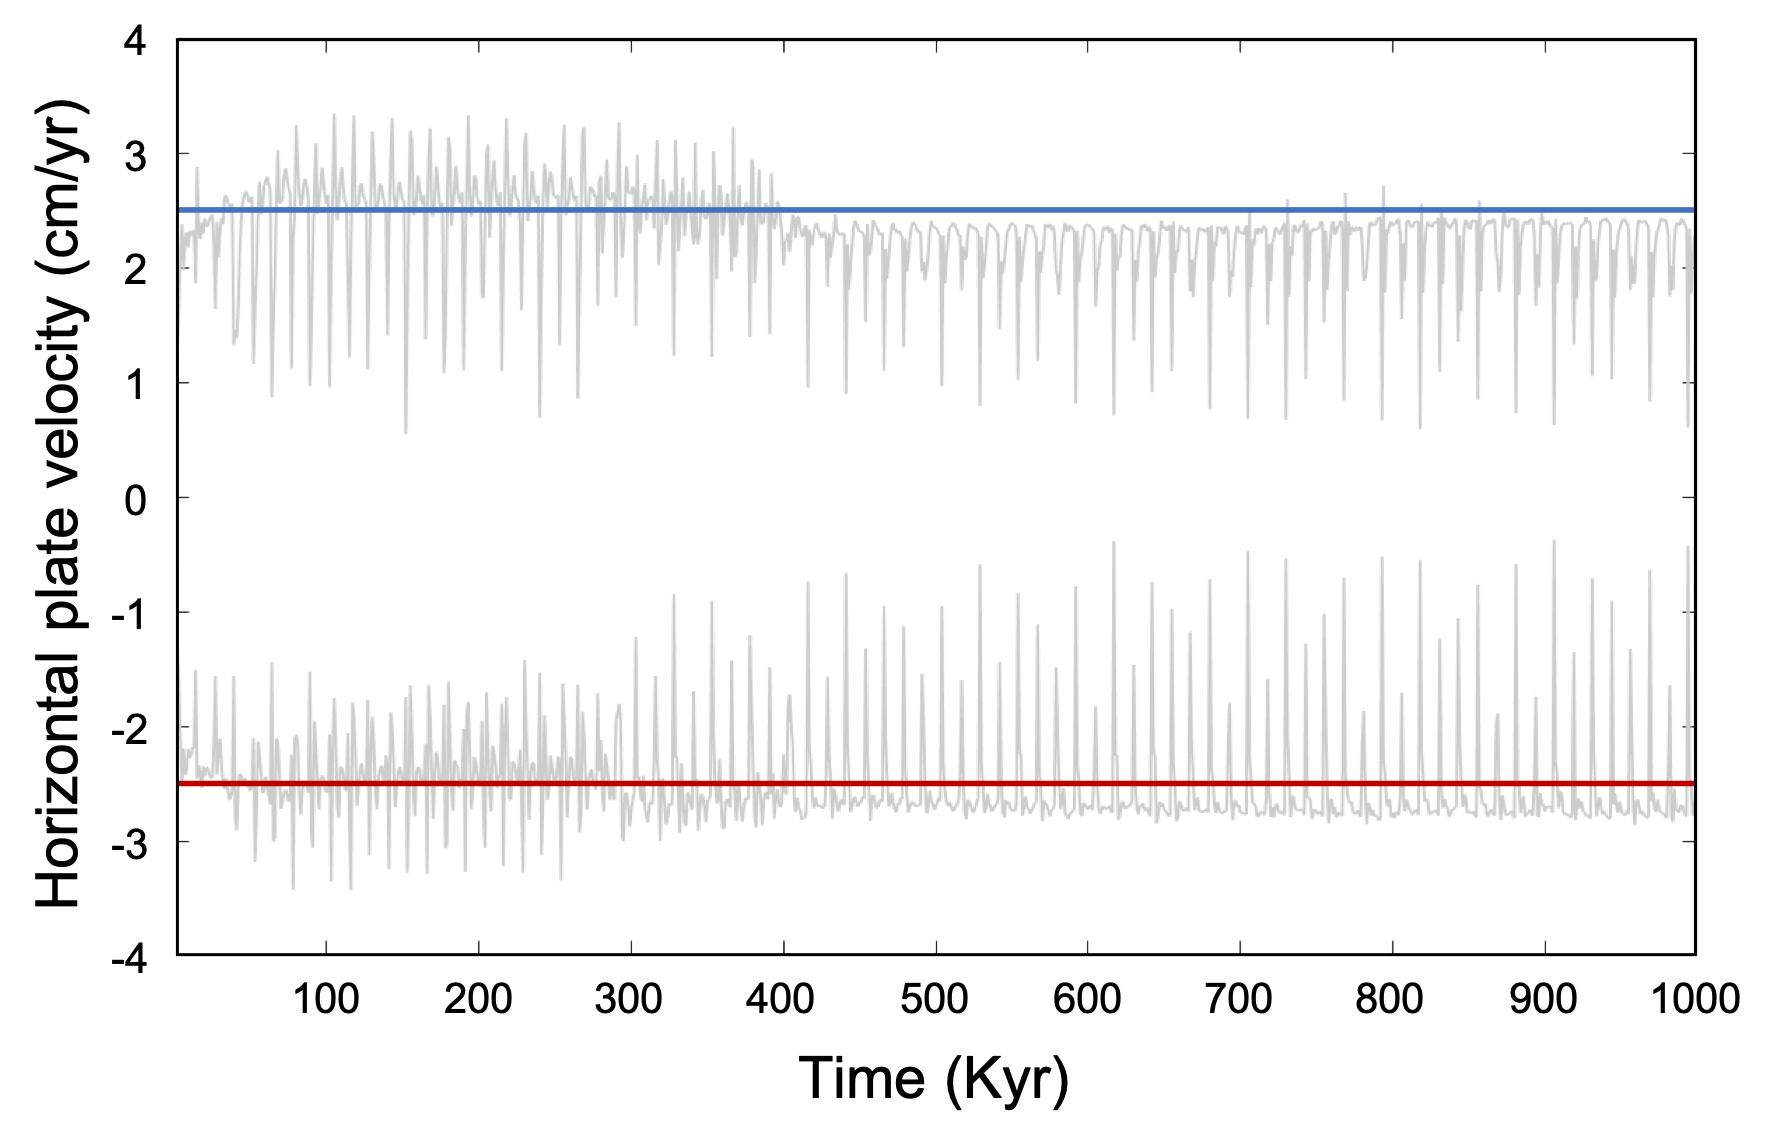
\includegraphics[width=0.9\linewidth]{./figs/f0m08to05.png}
	\caption{Horizontal plate velocity obtained from M=0.8 to 0.5 $(\boldsymbol{F_{res}})_x=0$ model. As a reference, 2.5 cm/yr and $-$2.5 cm/yr are plotted as blue and red lines.}
	\label{fig:f008to05}
\end{figure}

\section{Constant $(\boldsymbol{F_{bdy}})_x$ models}

This condition characterizes both $(\boldsymbol{F_{int}})_x$ and $(\boldsymbol{F_{res}})_x$ are dynamically changed by setting $(\boldsymbol{F_{bdy}})_x$ as a constant value. Since the net residual force keeps changing, plate velocity under this condition is continuously changing over time.

\subsection{Force balanced models}

Modeled fault behaviors from constant $(\boldsymbol{F_{bdy}})_x$ models are similar to that of kinematic models and  $(\boldsymbol{F_{res}})_x = 0$  models. For M = 0.5, a master detachment fault forms on one side (Figure \ref{fig:fbfault}A). In my model, the  faulting mode lasts until 650 Kyrs. For M = 0.8, the model produces a series of small-offset faults on both sides from the ridge axis (Figure \ref{fig:fbfault}B).

\begin{figure}[!htb]
	\centering
	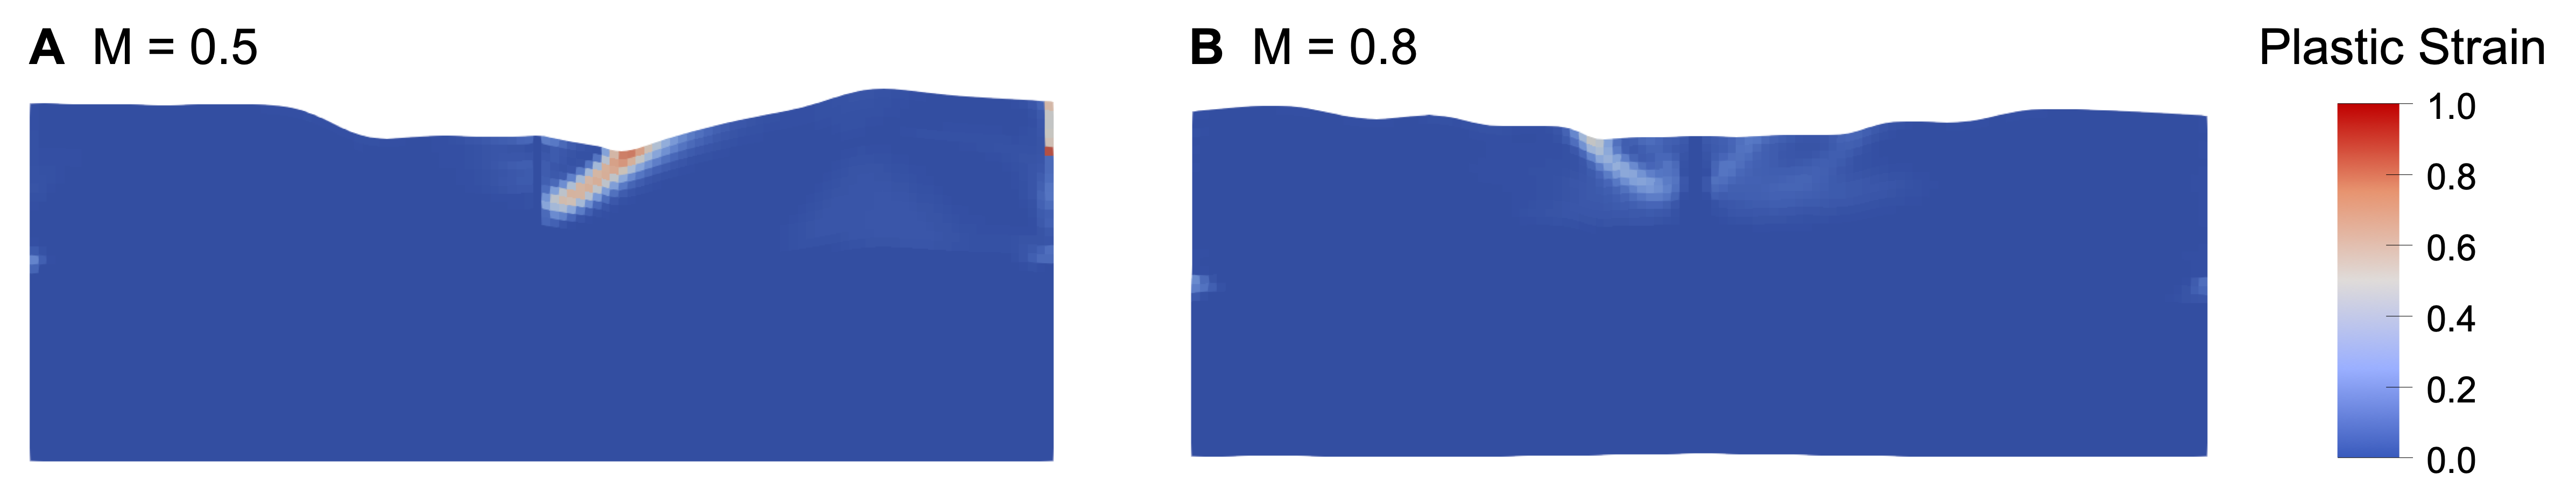
\includegraphics[width=0.99\linewidth]{./figs/fbfault.png}
	\caption{\textbf{A.} Snapshots of fault behavior of the constant $(\boldsymbol{F_{bdy}})_x$ model for M = 0.5 after 600 Kyrs. Model shows detachment faulting. \textbf{B.} Same as \textbf{A} but for M = 0.8 after 1 Myr. Model shows alternating faulting.}
	\label{fig:fbfault}
\end{figure}

Unlike above models, constant $(\boldsymbol{F_{bdy}})_x$ models show significant velocity changes over time. 
When M=0.5, the left-side plate velocity decrease stepwise from 2.7 cm/yr to 1 cm/yr and the right-side plate velocity decrease from 3 cm/yr to 2.5 cm/yr (Figure \ref{fig:m05vel}).
When M=0.8, both sides of plate velocities change more vigorously than other models (Figure \ref{fig:m08vel}). Until 250 Kyrs, the left-side plate velocity increase up to 3cm/yr, while the right-side plate velocity decrease down to 1.5 cm/yr. From 250 to 310 Kyrs, now the left-side plate moves slowly and the right-side plate moves rapidly. From 310 to 390 Kyrs, again the left plate velocity increase and the right plate velocity decrease. These velocity varying phases are repeated until the model ends.

%Unlike velocity-driven model, force-driven model shows significant velocity changes over time. The detachment fault forms at 50Kyrs on left side of the spreading axis. After *yrs, the left plate moves slowly.

\begin{figure}[!htb]
	\centering
	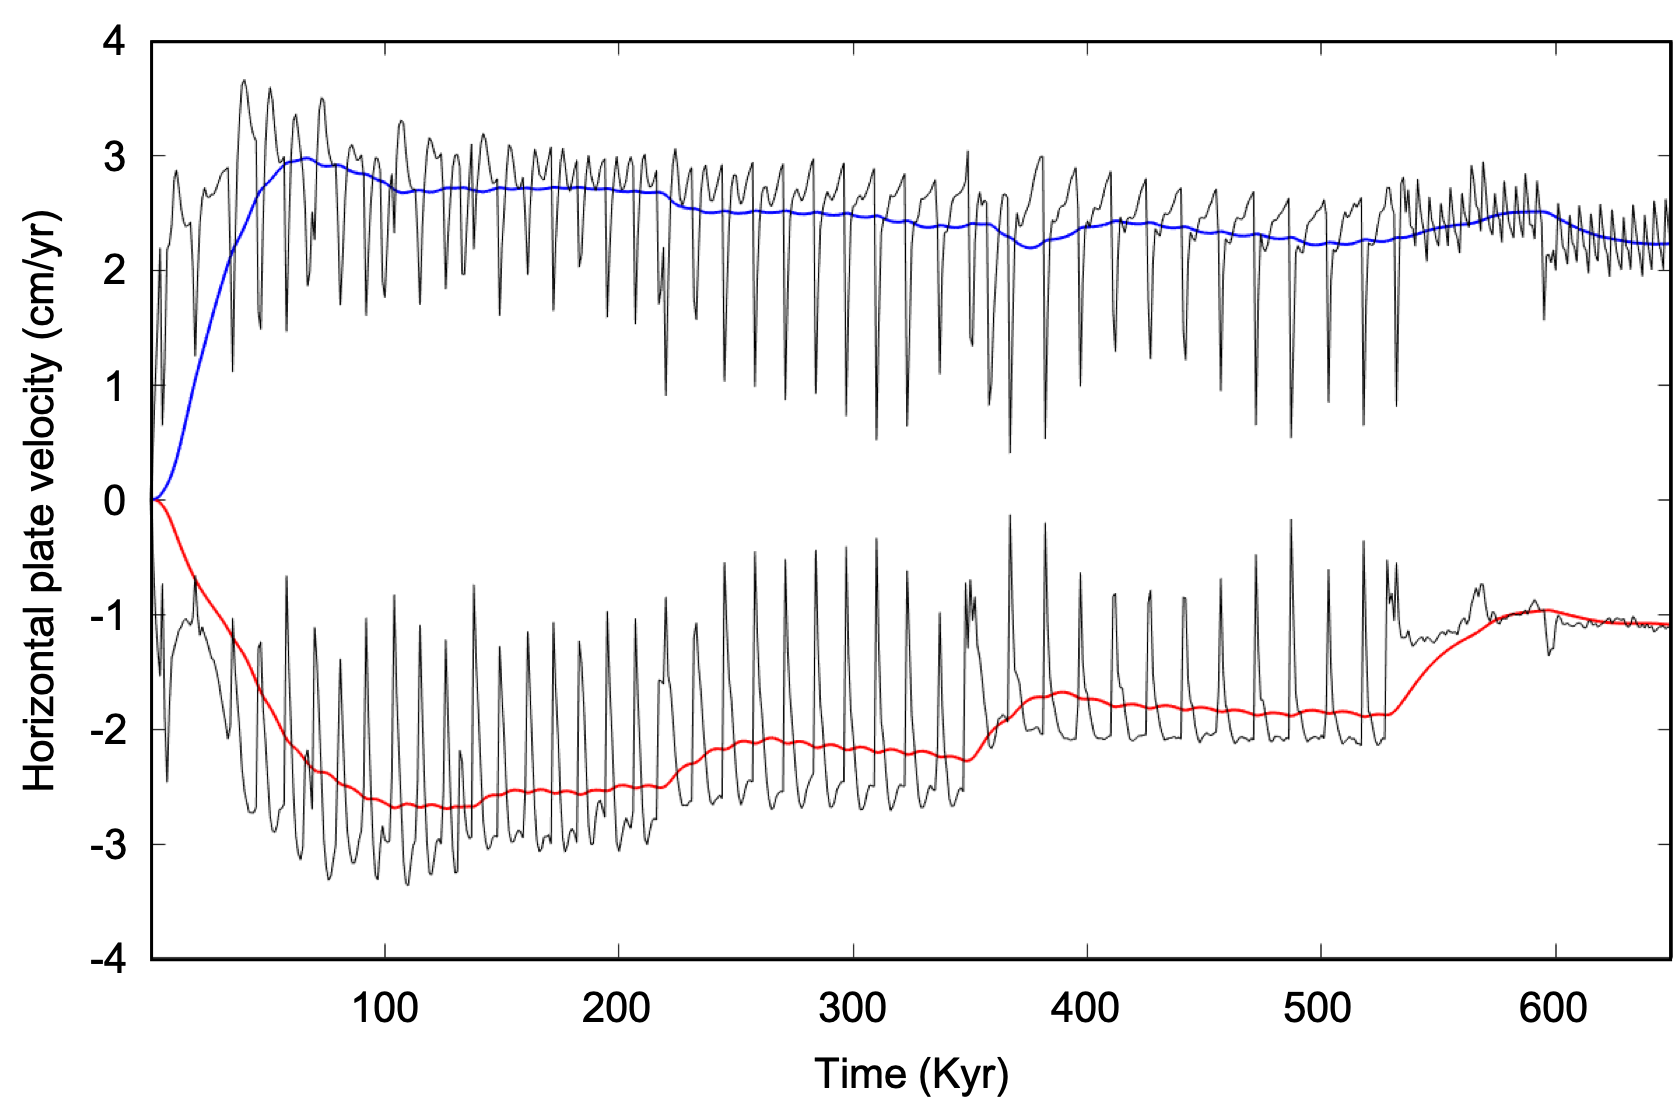
\includegraphics[width=0.9\linewidth]{./figs/m05vel.png}
	\caption{Plate velocity obtained from constant $(\boldsymbol{F_{bdy}})_x$ model results when M = 0.5. Abnormal peaks from remeshing effects are filtered out.}
	\label{fig:m05vel}
\end{figure}

%\subsubsection{M = 0.8}

%When $M=0.8$, fault migrates toward off-axis. The fault eventually becomes inactive and is replaced by new and near-axis fault.

\begin{figure}[!htb]
	\centering
	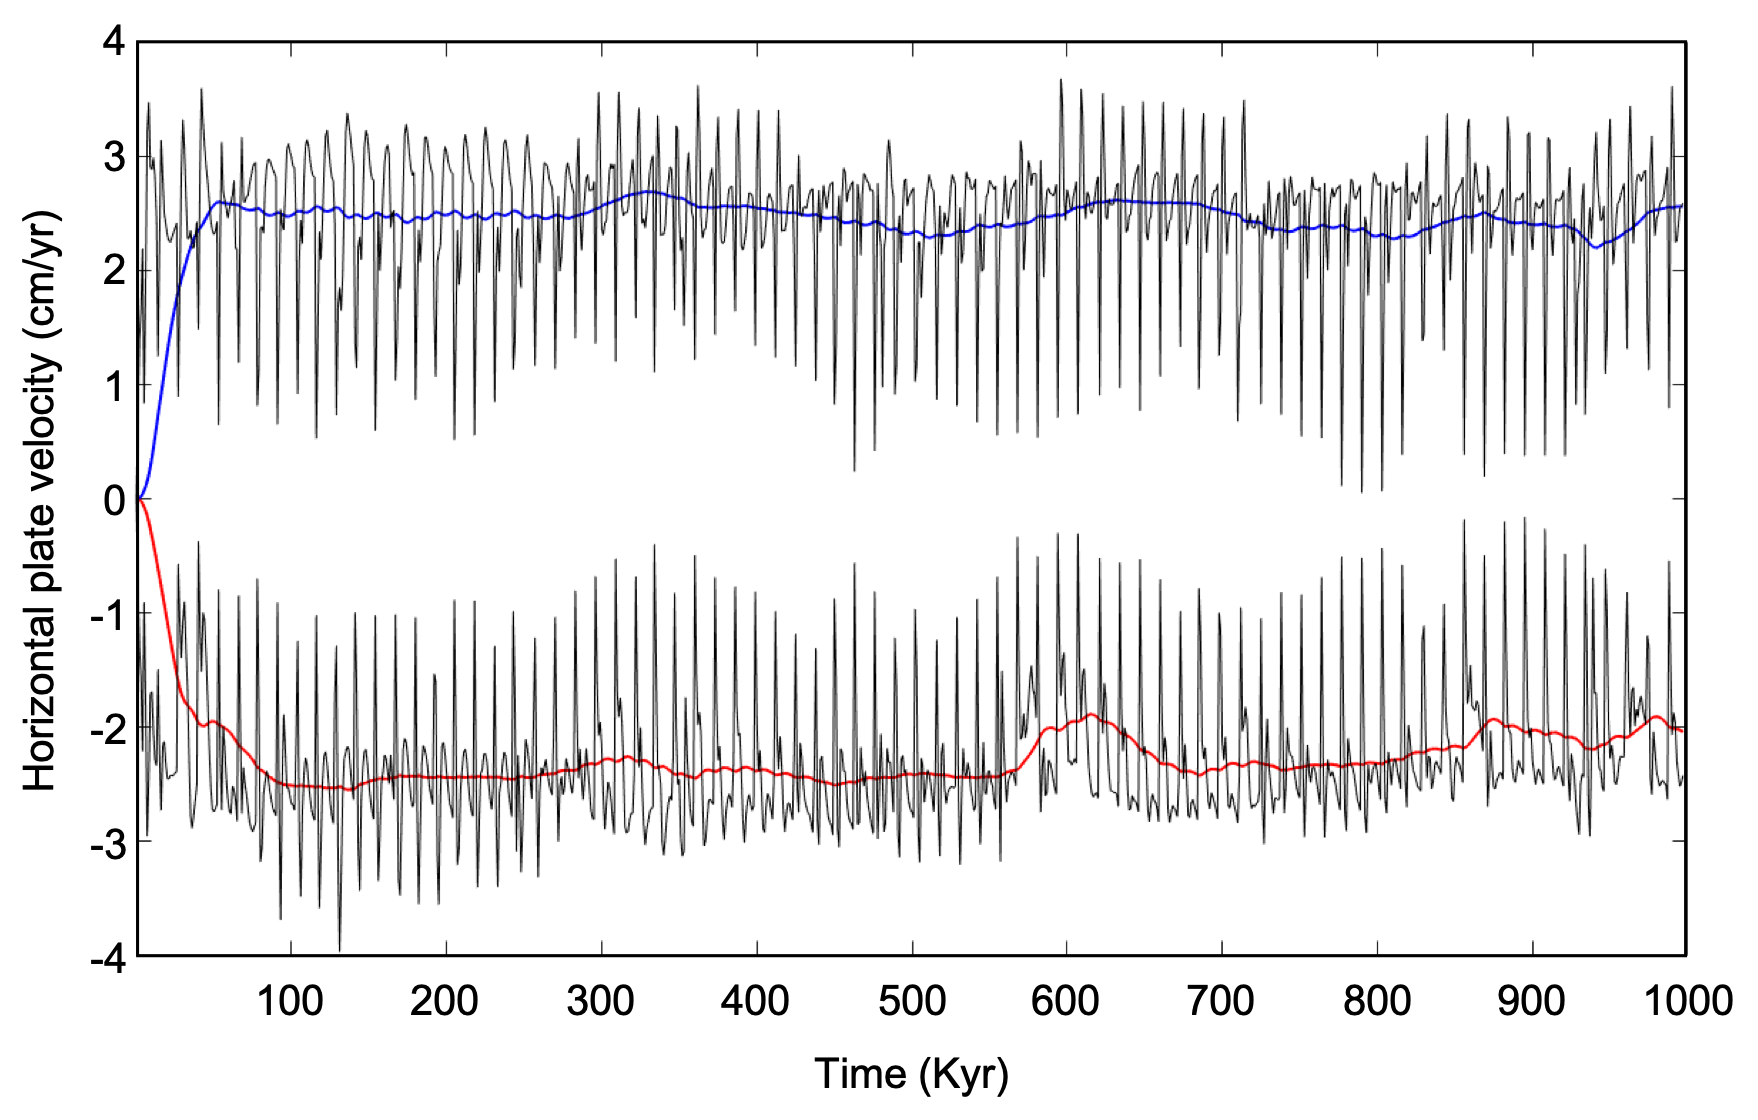
\includegraphics[width=0.9\linewidth]{./figs/m08vel.png}
	\caption{Plate velocity obtained from constant $(\boldsymbol{F_{bdy}})_x$ model results when M = 0.8. Abnormal peaks from remeshing effects are filtered out.} 
	\label{fig:m08vel}
\end{figure}

\subsection{Force balanced models with hotter mantle rheology}

Hotter mantle models show expected faulting modes for each M values. For M = 0.5, models produce one master detachment fault (Figure A). For M = 0.8, a series of small-offset faults on both sides form on both sides from the axis (Figure B).

Comparing to the constant $(\boldsymbol{F_{bdy}})_x$ models with normal mantle temperature, 

%Long term and large magnitude variation which cannot be explained by fault evolution may be caused by changes of the plate thermal state. By varying heat injection rate of the model, different behaviors of long term and large magnitude plate speed variation are observed. 

%\begin{table}[h!]
%	\centering
%	\caption{Percentage of P-wave and S-wave RMS reduction with respect to the original for different smoothing values after 20 iterations. The P-wave RMS reduction when using smoother = 10 is negative, which means that the inversion does not converge under this configuration.}
%	\label{tab:rms_reduction}
%	\begin{tabular}{ccc}
%		\toprule
%		Smoother & P-wave RMS reduction & S-wave RMS reduction \\
%		\midrule
%		10 & -14.7398\% & 9.9293\% \\
%		64 & 20.3963\% & 17.455\% \\
%		100 & 19.2424\% & 14.1327\% \\
%		128 & 17.3583\% & 7.5101\% \\
%		256 & 11.8203\% & 2.3572\% \\
%		\bottomrule
%	\end{tabular}
%\end{table}

\chapter{Discussion}

Results of horizontal plate velocities in kinematic models indicate that the fault development at a ridge affects plate velocity. In kinematic models, normal faults migrate away from the axis at a rate $2v_p($M$-0.5)$, where $v_p$ is a constant plate-driving velocity (Figure \ref{fig:hangingwall}) \citep{Buck2005}. The plate containing an active fault is slower than the other plate. When M = 0.5, A master detachment fault forms on one side and do not move and hence the plate velocities remain constant value, with one plate moves faster than another. When M = 0.8, faults initiate near the ridge axis and are rafted off-axis. The new fault is antithetic and forms on the opposite side of the ridge axis from the original fault. In this reason, the models have repeated two phase velocity corresponding to the alternating faulting mode.

\begin{figure}[!htb]
	\centering
	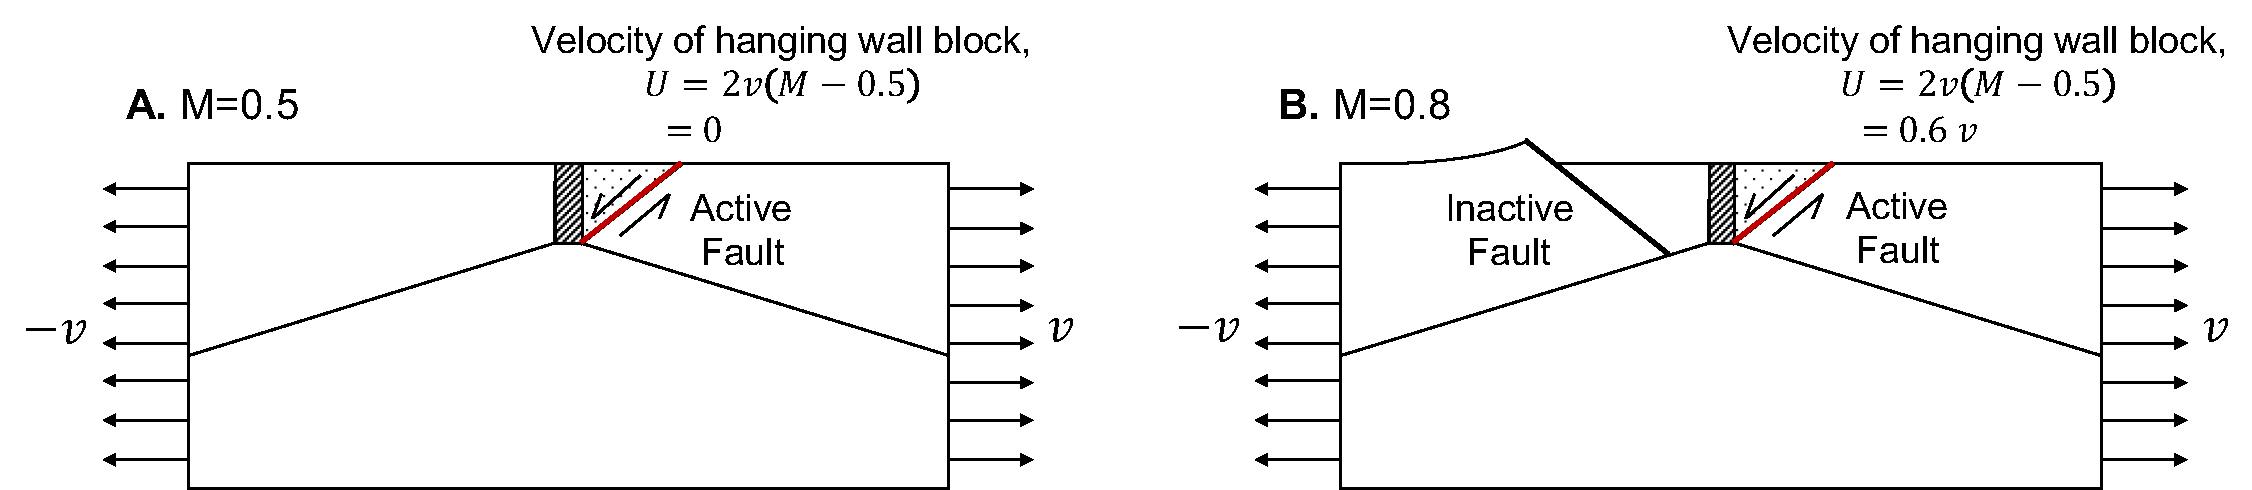
\includegraphics[width=0.99\linewidth]{./figs/hangingwall.pdf}
	\caption{\textbf{A.} Schematic model showing velocity of a plate including active fault at mid-ocean ridges driven by velocity when M = 0.5. \textbf{B.} Same as \textbf{A} but for M = 0.8.}
	\label{fig:hangingwall}
\end{figure}


Similarly, in the cases of force-driven model, interaction between dynamic driving velocity from boundary force and opposite direction velocity from normal faults controls the plate speed in force.
When half of total plate growth is accommodated by magma intrusion at spreading center, the velocity of one plate is always lower than another. Models produce repeated pattern of two-phase plate velocity when most of total plate spreading is taken up by dike.

Besides these velocity variations, another fluctuation with greater amplitude and frequency is observed in constant $(\boldsymbol{F_{bdy}})_x$ models. Fault evolution is not sufficient to explain this long term and large magnitude variation. This fluctuation may come from the deep interior, as the feedback between deep mantle dynamics and surface plate motion. Hotter mantle conditioned models 

\chapter{Conclusion}

\bibliography{references}     % before changing bibliographystyle, remove *.bbl files in your working directory
\bibliographystyle{agsm.bst}  % the closest style to the University of Memphis Thesis Style Guide

\end{document}
